\documentclass[10pt,a4paper]{article}
\usepackage[margin=1.8cm]{geometry}
\usepackage[utf8]{inputenc}
\usepackage[T1]{fontenc}
\usepackage{booktabs}
\usepackage{multicol}
\usepackage{multirow}
\usepackage{parskip}
\usepackage{xcolor}
\usepackage{array}
\usepackage{graphicx}
\usepackage{colortbl}
\usepackage{hyperref}

\graphicspath{{figures/}}

\setlength{\parskip}{3pt}
\setlength{\columnsep}{1cm}

\title{\textbf{Pipeline Results Summary}\\
\large AI Coding Agent Adoption in JS/TS/npm Repositories on GitHub\\[2pt]
\normalsize Manuel Youssef Haik Kevorkian}
\date{November 2026 \quad \textcolor{red}{\textbf{DRAFT -- not for submission}}}

\begin{document}
\maketitle
\vspace{-4pt}
\hrule
\vspace{8pt}

% ─── STAGE 1 ──────────────────────────────────────────────────────────────────
\section*{Stage 1 --- Corpus Construction}

\begin{multicols}{2}

\textbf{Corpus:} 60,129 repositories created after 24 Feb 2025, JS+TS bytes
$\geq 175{,}000$, $\geq 4$ stars, $\geq 50$ commits, not a fork.

\begin{tabular}{@{}lrr@{}}
\toprule
Ecosystem & Repos & \% \\
\midrule
npm           & 28,248 & 47.0 \\
pnpm          & 12,229 & 20.3 \\
vanilla       & 10,177 & 16.9 \\
npm\_no\_lock &  7,979 & 13.3 \\
yarn          &  1,091 &  1.8 \\
deno          &    250 &  0.4 \\
bun           &    107 &  0.2 \\
\midrule
\textbf{Total} & \textbf{60,129} & \textbf{100.0} \\
\bottomrule
\end{tabular}

\columnbreak

\textbf{Language split:} TypeScript 45,314 (75.4\%) \quad JavaScript 14,815 (24.6\%)

\vspace{6pt}
% ─── STAGE 2 ────────────────────────────────────────────────────────────────
\section*{Stage 2 --- Owner Location Inference}

\begin{tabular}{@{}lrr@{}}
\toprule
Pass & Owners & Cumul.\ \% \\
\midrule
Pass 1 (location field)            & 13,625 & 27.2 \\
Pass 2 (bio, TLD, network)         &  8,323 & 43.9 \\
Pass 3 (Nominatim + TZ + script)   &  6,266 & 56.4 \\
Pass 4 (company ROR + org orgs)    &     65 & 56.6 \\
\midrule
Located total              & 28,279 & 56.6 \\
Not specified              & 21,723 & 43.4 \\
\textbf{Unique owners}     & \textbf{50,002} & \\
\bottomrule
\end{tabular}

Top countries: China 5,829 (20.6\%), US 3,981 (14.1\%), India 3,945 (14.0\%)
\end{multicols}

\vspace{4pt}
\begin{center}
  \begin{minipage}[t]{0.47\textwidth}
    \centering
    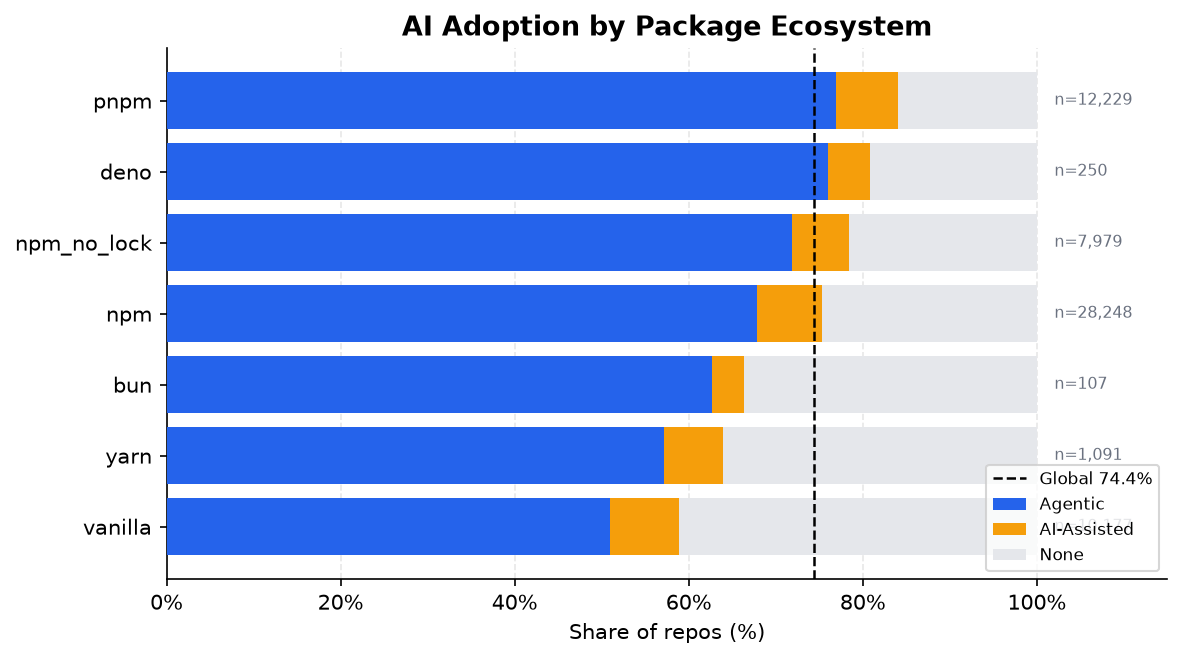
\includegraphics[width=\linewidth]{fig_ecosystem_stacked.png}\\
    \small\textit{Stage 1 --- Package ecosystem distribution}
  \end{minipage}
  \hfill
  \begin{minipage}[t]{0.47\textwidth}
    \centering
    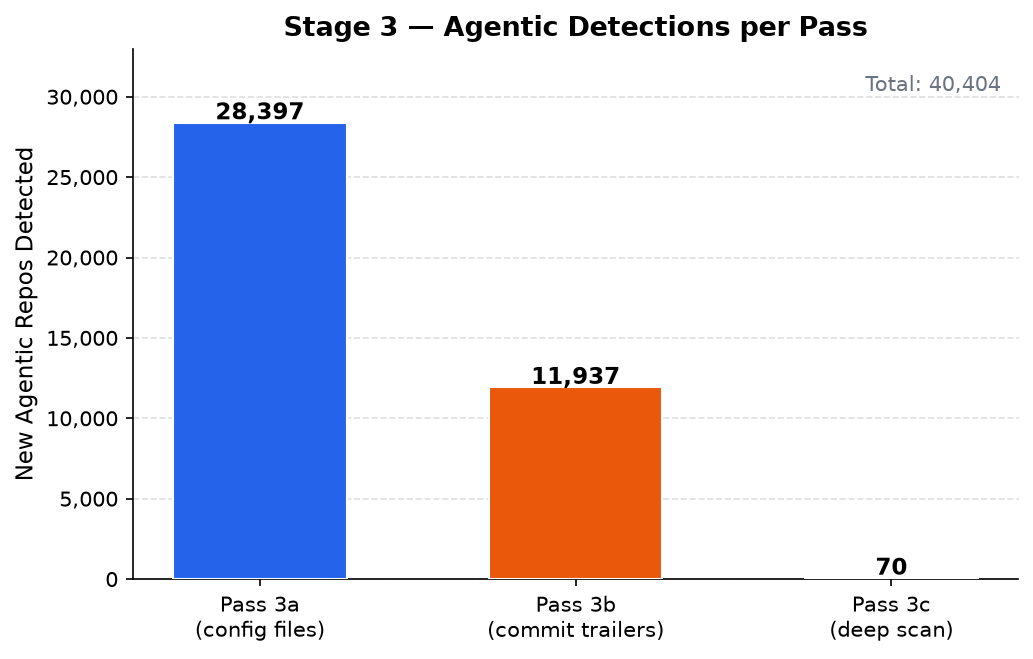
\includegraphics[width=\linewidth]{fig_pass_contributions.png}\\
    \small\textit{Stage 3 --- Agentic detections per pass}
  \end{minipage}
\end{center}

\vspace{6pt}
\hrule
\vspace{6pt}

% ─── STAGE 3 ──────────────────────────────────────────────────────────────────
\section*{Stage 3 --- AI Adoption Detection (Three Passes)}

\begin{multicols}{2}

\begin{tabular}{@{}lrr@{}}
\toprule
Pass & Agentic & Input \\
\midrule
Pass 3a --- config files    & 28,397 (47.2\%) & 60,129 \\
Pass 3b --- commit trailers & 11,937 (37.6\%) & 31,732 \\
Pass 3c --- deep scan       & 70 agentic; 4,397 AI-asst & 19,795 \\
\bottomrule
\end{tabular}

\textbf{Pass 3a top agents:}\\
Claude Code \quad 18,313 (64.5\% of pass)\\
Generic \quad 17,015 (59.9\%)\\
Cursor \quad 2,247 (7.9\%)\\
GitHub Copilot \quad 1,798 (6.3\%)

\columnbreak

\textbf{Final Classification:}

\begin{tabular}{@{}lrr@{}}
\toprule
Label & Repos & \% \\
\midrule
Agentic      & 40,364 & 67.1 \\
AI-assisted  &  4,397 &  7.3 \\
None         & 15,368 & 25.6 \\
\midrule
\textbf{Total adopted} & \textbf{44,761} & \textbf{74.4} \\
\textbf{Total corpus}  & \textbf{60,129} & \textbf{100.0} \\
\bottomrule
\end{tabular}

\vspace{4pt}
\textbf{Breakdowns:}\\
TypeScript 78.5\% \quad JavaScript 62.0\%\\
pnpm 84.0\% \quad npm 75.3\% \quad vanilla 58.9\%\\[3pt]
\textbf{Tool loyalty:} 66.3\% of adopters use 1 tool\\
Claude Code only: 34.4\% of adopters\\
Top pair: Claude Code + Generic (9,245 repos, 20.7\%)
\end{multicols}

\vspace{4pt}
\begin{center}
  \begin{minipage}[t]{0.47\textwidth}
    \centering
    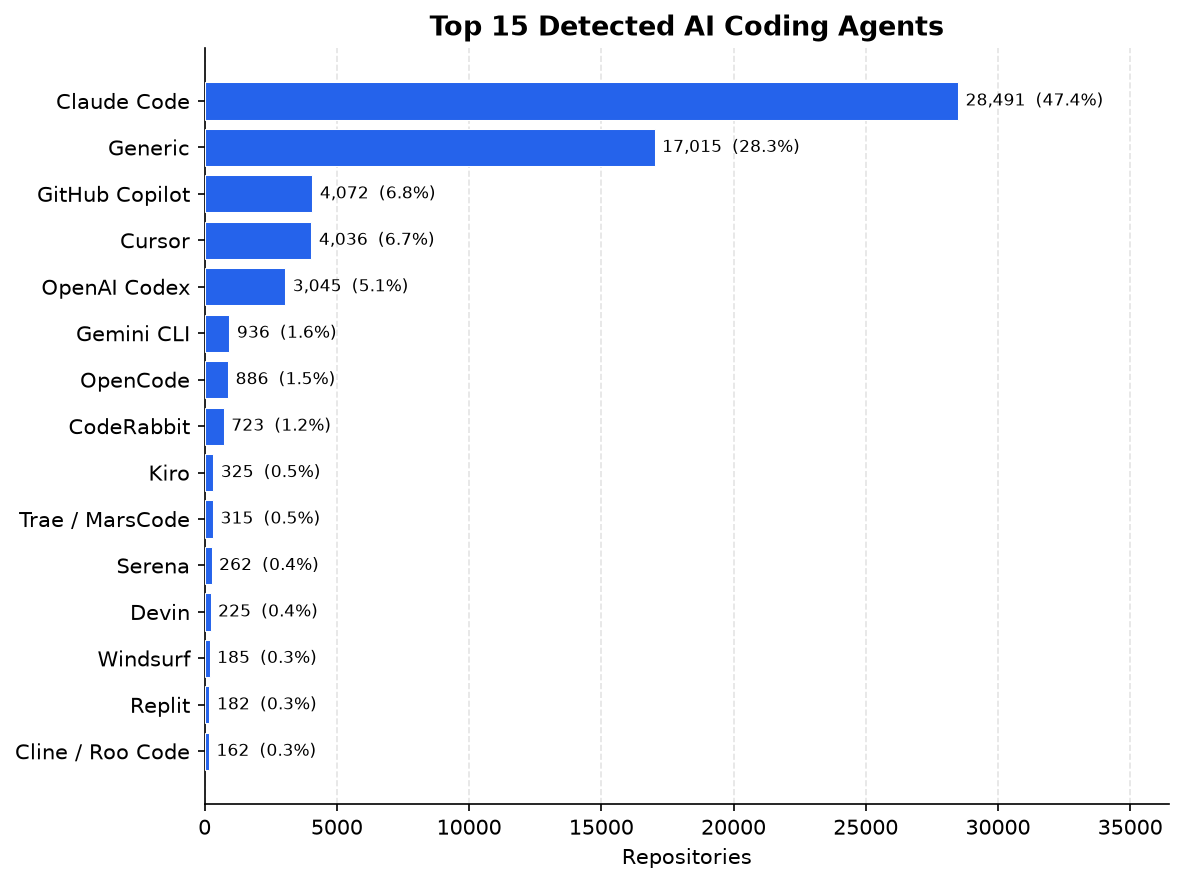
\includegraphics[width=\linewidth]{fig_tool_distribution.png}\\
    \small\textit{Stage 3 --- Agent tool distribution (top 15)}
  \end{minipage}
  \hfill
  \begin{minipage}[t]{0.47\textwidth}
    \centering
    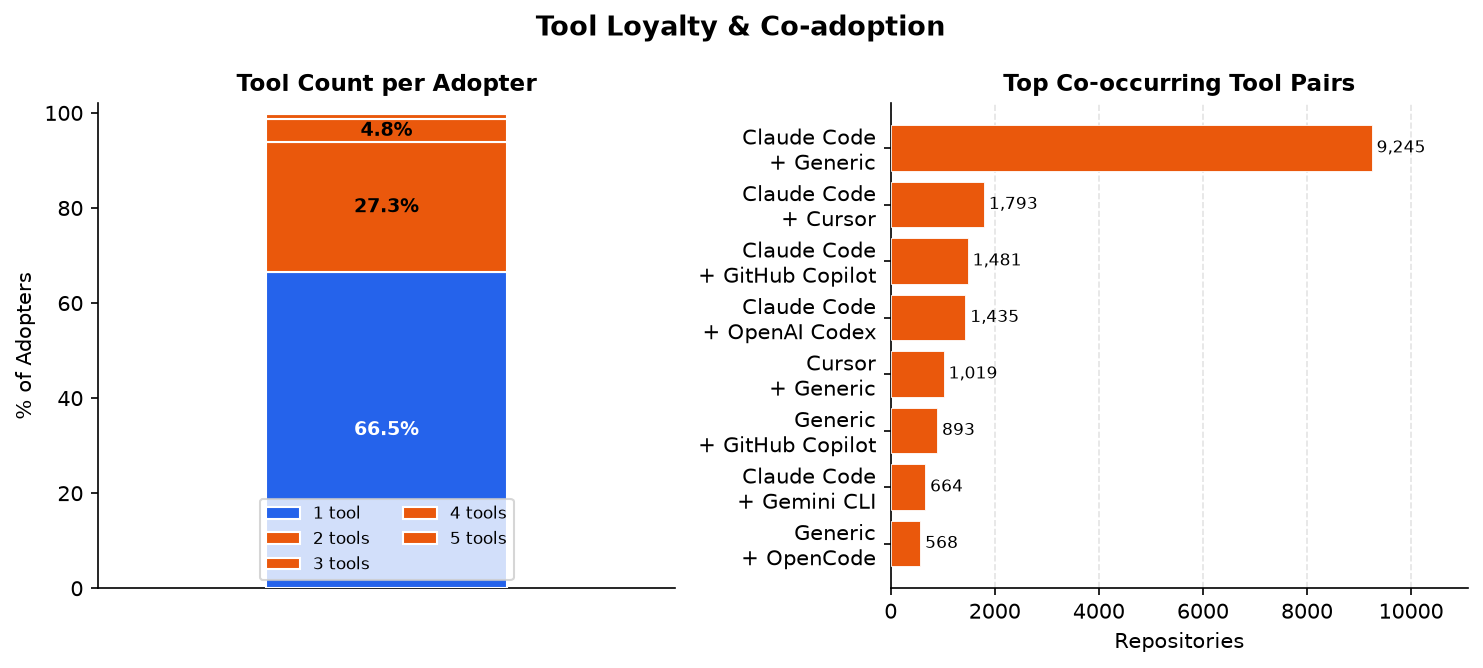
\includegraphics[width=\linewidth]{fig_tool_loyalty.png}\\
    \small\textit{Stage 3 --- Tool loyalty (single vs multi-tool) and top pairs}
  \end{minipage}
\end{center}

\vspace{6pt}
\hrule
\vspace{6pt}

\newpage
% ─── STAGE 4 ──────────────────────────────────────────────────────────────────
\section*{Stage 4 --- Geographic Analysis}

\textbf{Coverage:} 66 countries with $\geq 30$ repos \quad
33,848 repos with country (56.3\% of corpus) \quad
Global adoption rate: \textbf{74.4\%} \quad Wilson 95\% CI: [74.09\%, 74.79\%]

\begin{multicols}{2}

\textbf{Top 10 countries:}

\begin{tabular}{@{}rlrr@{}}
\toprule
Rk & Country & Repos & Rate\% \\
\midrule
 1 & Saudi Arabia  &    33 & 90.9* \\
 2 & Belgium       &    94 & 90.4* \\
 3 & UAE           &   119 & 87.4* \\
 4 & South Korea   &   786 & 86.9* \\
 5 & Taiwan        &   326 & 85.0* \\
 6 & Israel        &   192 & 84.9* \\
 7 & Malaysia      &    92 & 83.7* \\
 8 & Denmark       &   115 & 83.5* \\
 9 & United States & 4,926 & 82.9* \\
10 & Sweden        &   205 & 82.9* \\
\bottomrule
\end{tabular}

\columnbreak

\textbf{Bottom 10 countries:}

\begin{tabular}{@{}rlrr@{}}
\toprule
Rk & Country & Repos & Rate\% \\
\midrule
57 & Nigeria    &   270 & 47.4* \\
58 & Iran       &   287 & 46.3* \\
59 & Pakistan   &   275 & 44.7* \\
60 & Ghana      &    40 & 42.5* \\
61 & Morocco    &    81 & 38.3* \\
62 & Kenya      &   164 & 37.8* \\
63 & Ethiopia   &   102 & 37.2* \\
64 & Nepal      &   105 & 35.2* \\
65 & Sri Lanka  &   107 & 34.6* \\
66 & Rwanda     &    51 & 27.5* \\
\bottomrule
\end{tabular}

\end{multicols}

\vspace{4pt}
\begin{center}
  \begin{minipage}[t]{0.47\textwidth}
    \centering
    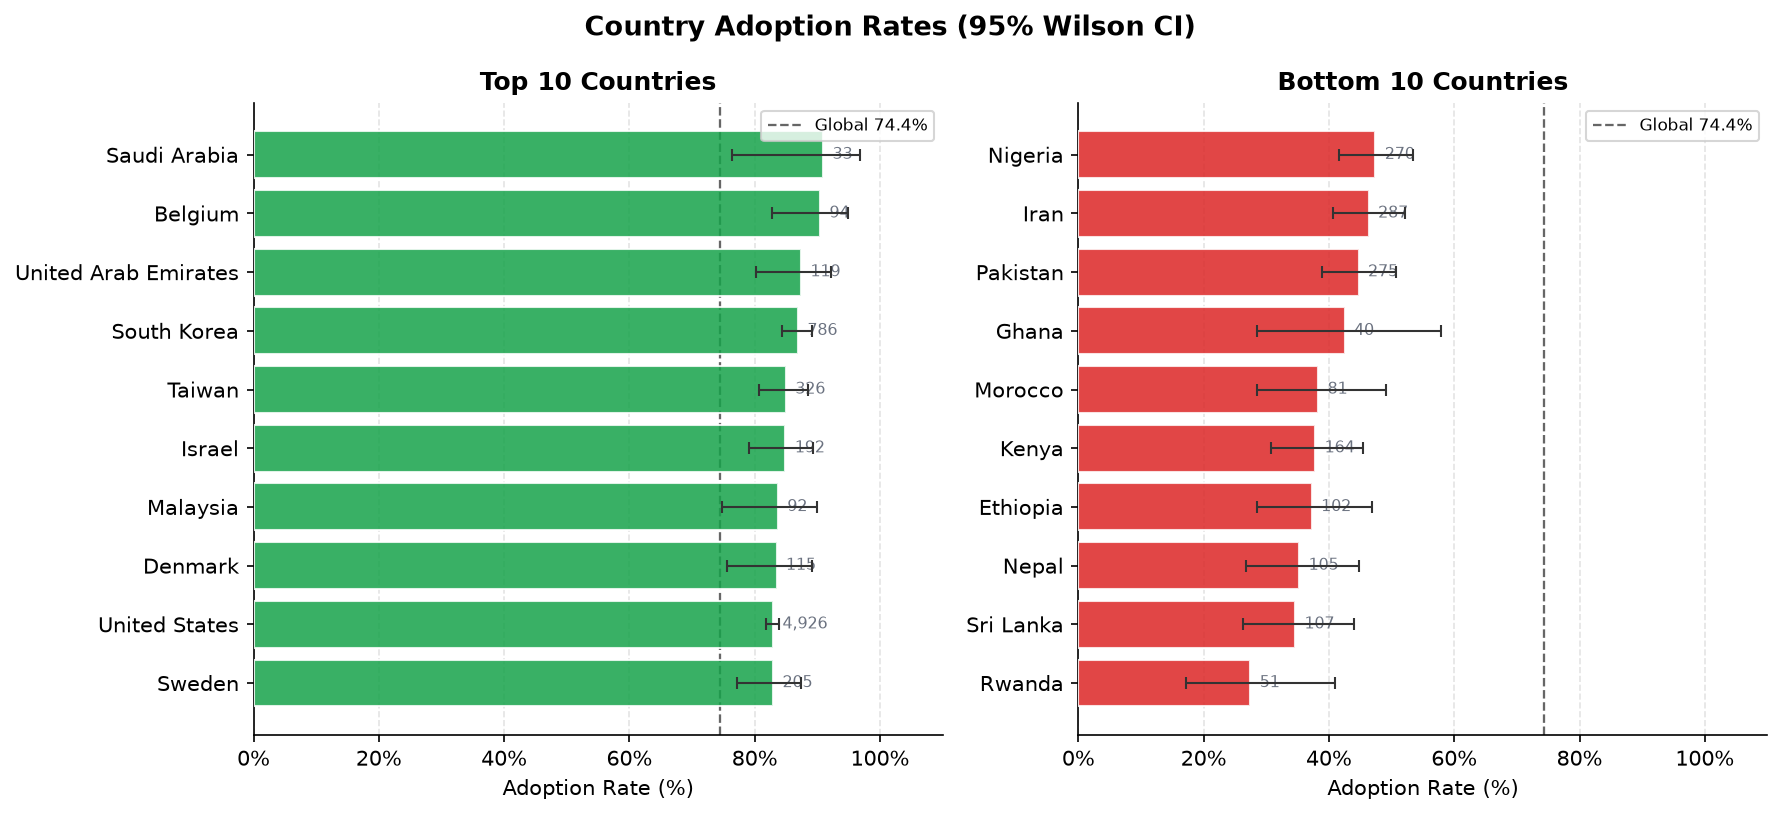
\includegraphics[width=\linewidth]{fig_top_bottom_countries.png}\\
    \small\textit{Top 10 vs bottom 10 countries by adoption rate (95\% Wilson CI)}
  \end{minipage}
  \hfill
  \begin{minipage}[t]{0.47\textwidth}
    \centering
    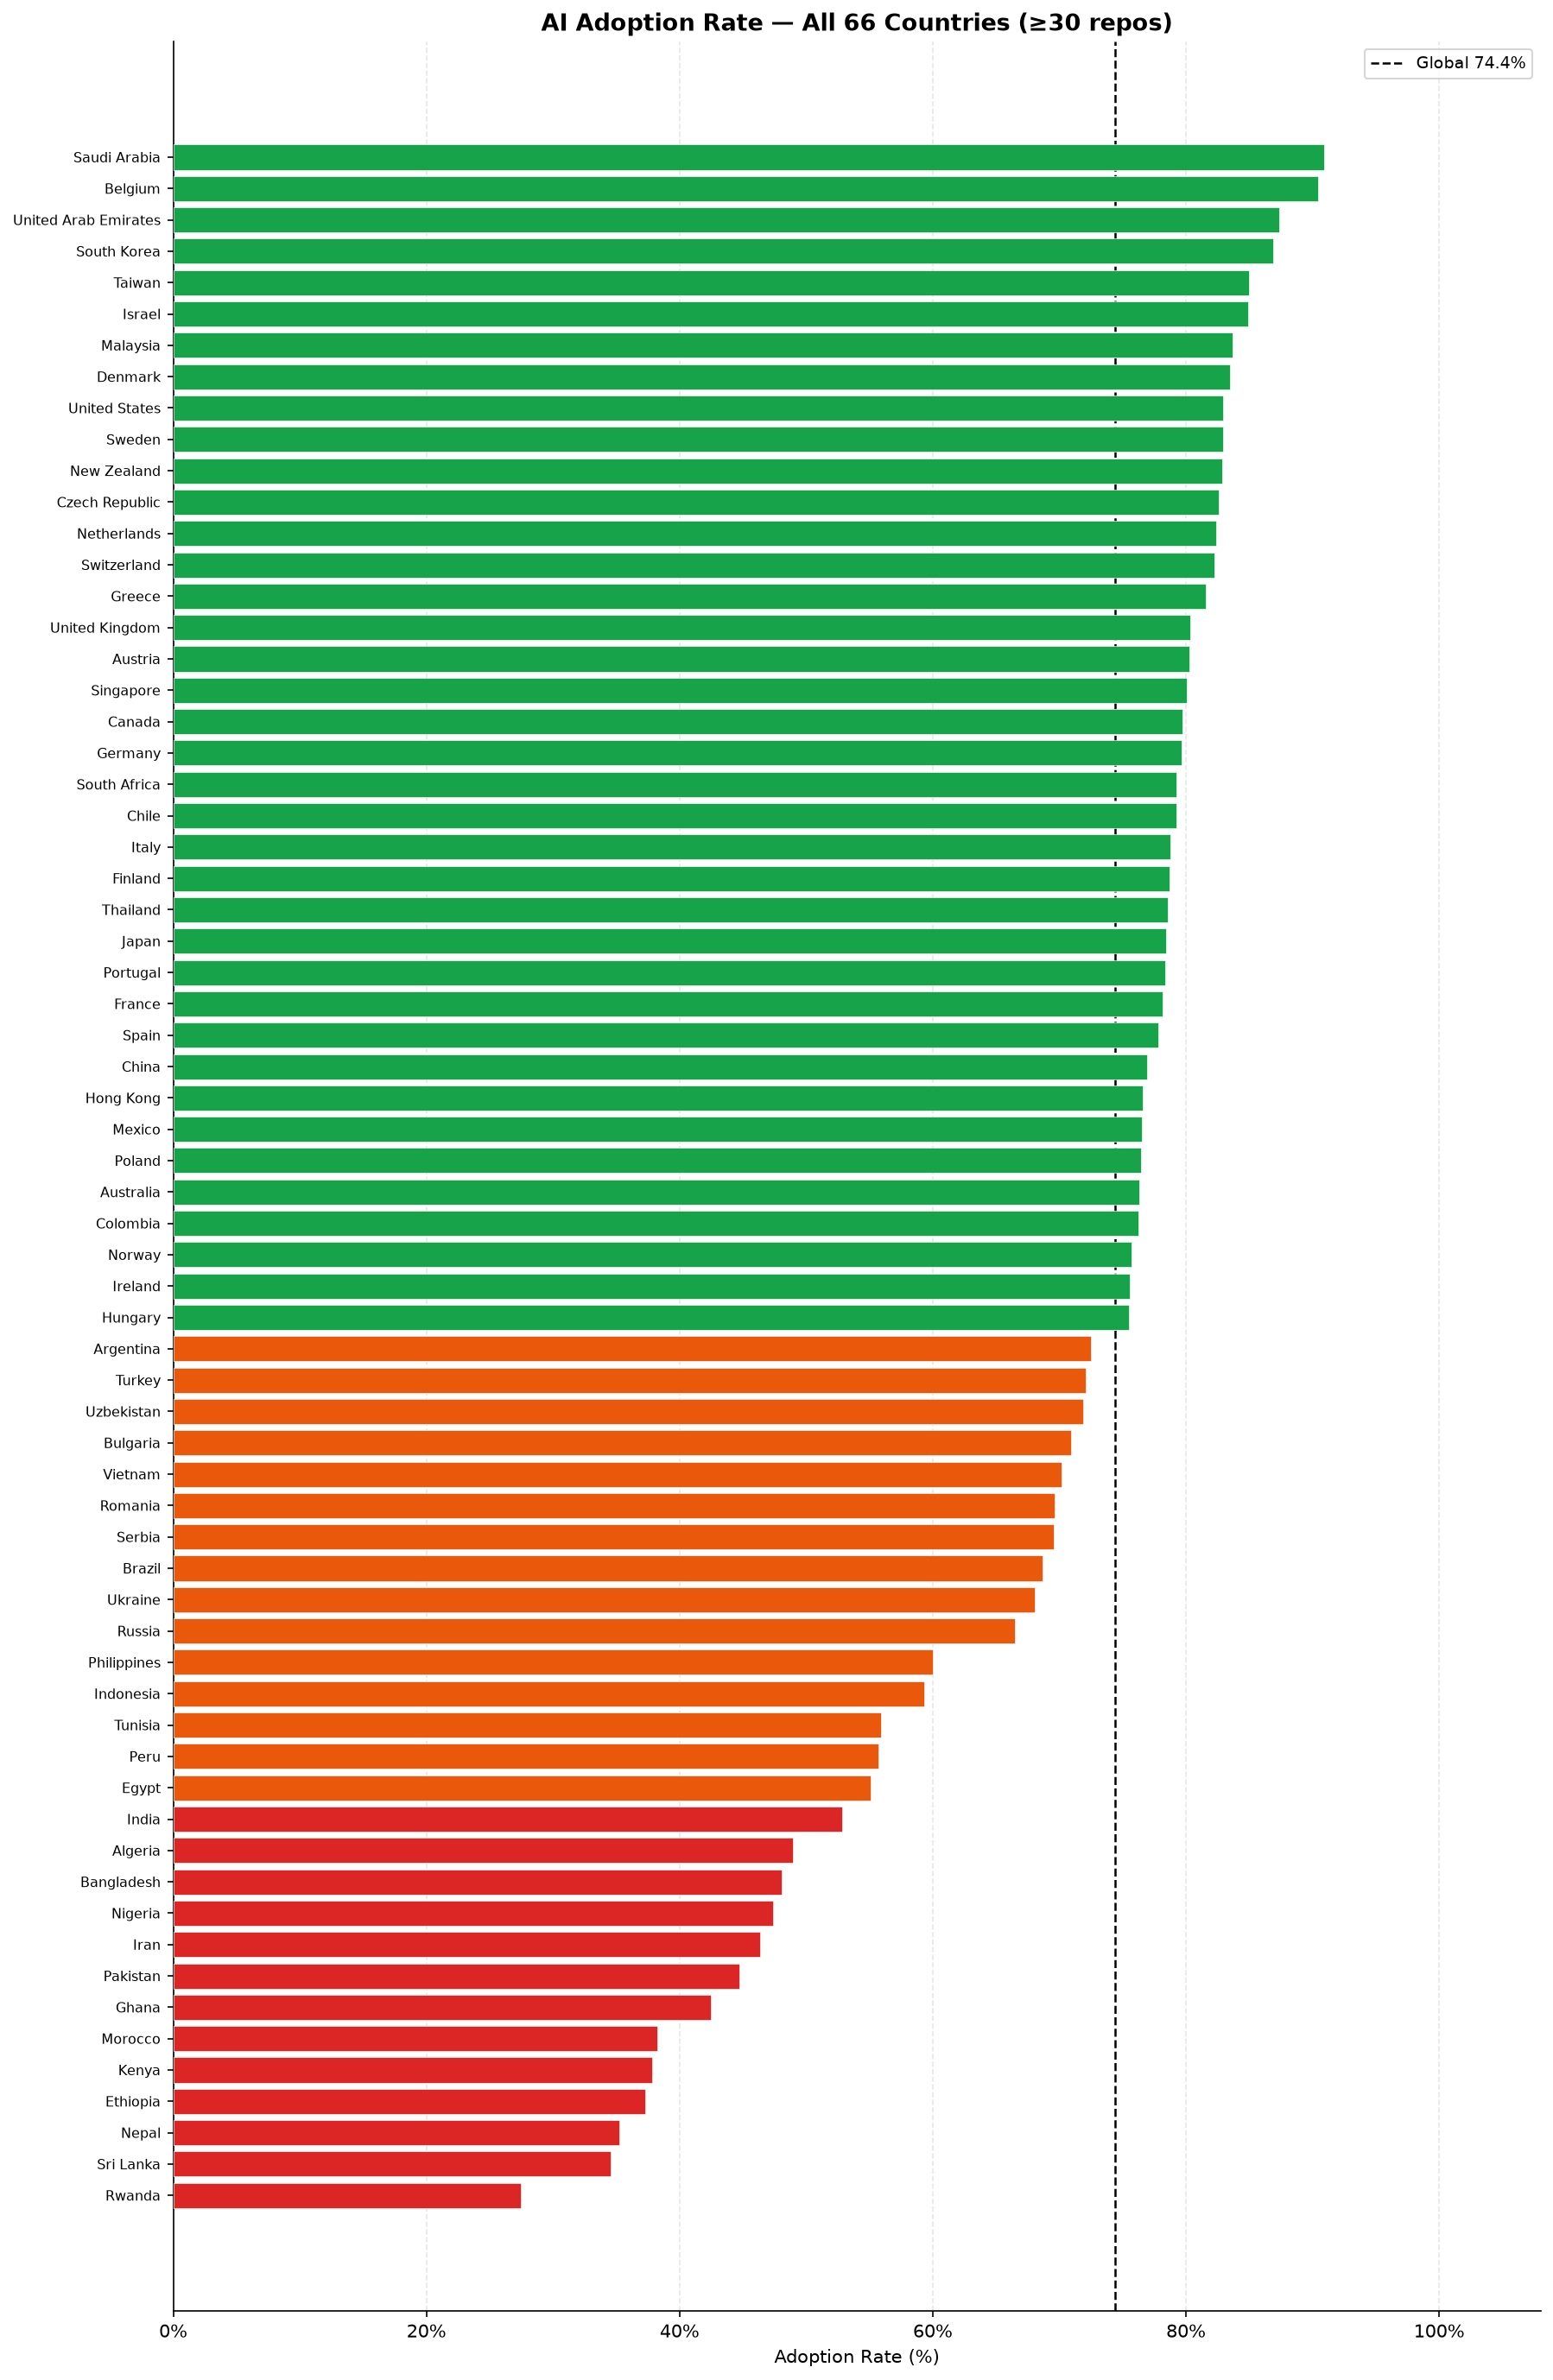
\includegraphics[width=\linewidth]{fig_choropleth.png}\\
    \small\textit{All 66 eligible countries sorted by adoption rate}
  \end{minipage}
\end{center}

\vspace{6pt}
\hrule
\vspace{6pt}

% ─── CLASSIFICATION LABELS ────────────────────────────────────────────────────
\section*{Classification Labels --- What Each Label Means}

\begin{multicols}{2}

\begin{tabular}{@{}lrrp{4.2cm}@{}}
\toprule
Label & Repos & \% & Condition \\
\midrule
Agentic     & 40,364 & 67.1 &
  $\geq$1 STRONG signal \emph{or} $\geq$2 MEDIUM families \\[2pt]
AI-assisted &  4,397 &  7.3 &
  1 MEDIUM only \emph{or} WEAK only, configured but unconfirmed \\[2pt]
None        & 15,368 & 25.6 &
  No signal found in any of the three passes \\
\bottomrule
\end{tabular}

\columnbreak

\textbf{STRONG} (agent \emph{did} work):\\
bot\_author, ci\_workflow, pr\_branch,\\
agent\_attribution (commit trailers).\\[4pt]
\textbf{MEDIUM} (agent \emph{configured}):\\
config\_file (CLAUDE.md, .cursorrules\ldots), pr\_label.\\[4pt]
\textbf{WEAK} (incidental mention):\\
pr\_body, editor\_config.\\[4pt]
\textbf{AI-assisted} = evidence present but unconfirmed.
Included in 74.4\% total; \textbf{67.1\% agentic-only}
is the conservative figure.

\end{multicols}

\vspace{6pt}
\noindent\textbf{Signal strength hierarchy:}
\vspace{4pt}

\noindent
\renewcommand{\arraystretch}{1.35}
\begin{tabular}{@{}
  >{\centering\arraybackslash\columncolor{red!18}}p{5.2cm}
  >{\centering\arraybackslash\columncolor{yellow!35}}p{5.2cm}
  >{\centering\arraybackslash\columncolor{gray!18}}p{5.2cm}@{}}
\textbf{STRONG} --- agent \emph{did} work &
\textbf{MEDIUM} --- agent \emph{configured} &
\textbf{WEAK} --- incidental mention \\[2pt]
\small\texttt{bot\_author} &
\small\texttt{config\_file} (CLAUDE.md, .cursorrules) &
\small\texttt{pr\_body} \\
\small\texttt{ci\_workflow} &
\small\texttt{pr\_label} &
\small\texttt{editor\_config} \\
\small\texttt{pr\_branch} & & \\
\small\texttt{agent\_attribution} (trailers) & & \\
\end{tabular}
\renewcommand{\arraystretch}{1}

\vspace{6pt}
\hrule
\vspace{6pt}

\newpage
% ─── THREE SIZING APPROACHES ──────────────────────────────────────────────────
\section*{Repository Size \& Adoption --- Three Operationalisations}

All three confirm the same monotonic pattern. B and C use corpus tertiles
(P33/P66) so each stratum holds $\approx$33\% of repos.

\vspace{3pt}
\begin{tabular}{@{}p{6.2cm}rrrr@{}}
\toprule
Approach & Small & Medium & Large & Range \\
\midrule
\textbf{A: Stars} ($\leq$50 / 51--500 / $>$500)
  \newline {\footnotesize repos: 49,562 \quad 8,375 \quad 2,192}
  & 72.1\% & 83.7\% & 92.2\% & $+$20.1\,pp \\[5pt]
\textbf{B: Commits} ($\leq$114 / 115--286 / $>$286)
  \newline {\footnotesize repos: 19,891 \quad 19,863 \quad 20,375}
  & 66.9\% & 75.0\% & 81.3\% & $+$14.4\,pp \\[5pt]
\textbf{C: Code volume} ($\leq$0.50\,MB / 0.50--1.45\,MB / $>$1.45\,MB)
  \newline {\footnotesize repos: 19,843 \quad 19,842 \quad 20,444}
  & 61.6\% & 74.8\% & 86.6\% & $+$25.0\,pp \\
\bottomrule
\end{tabular}

\vspace{4pt}
\begin{center}
  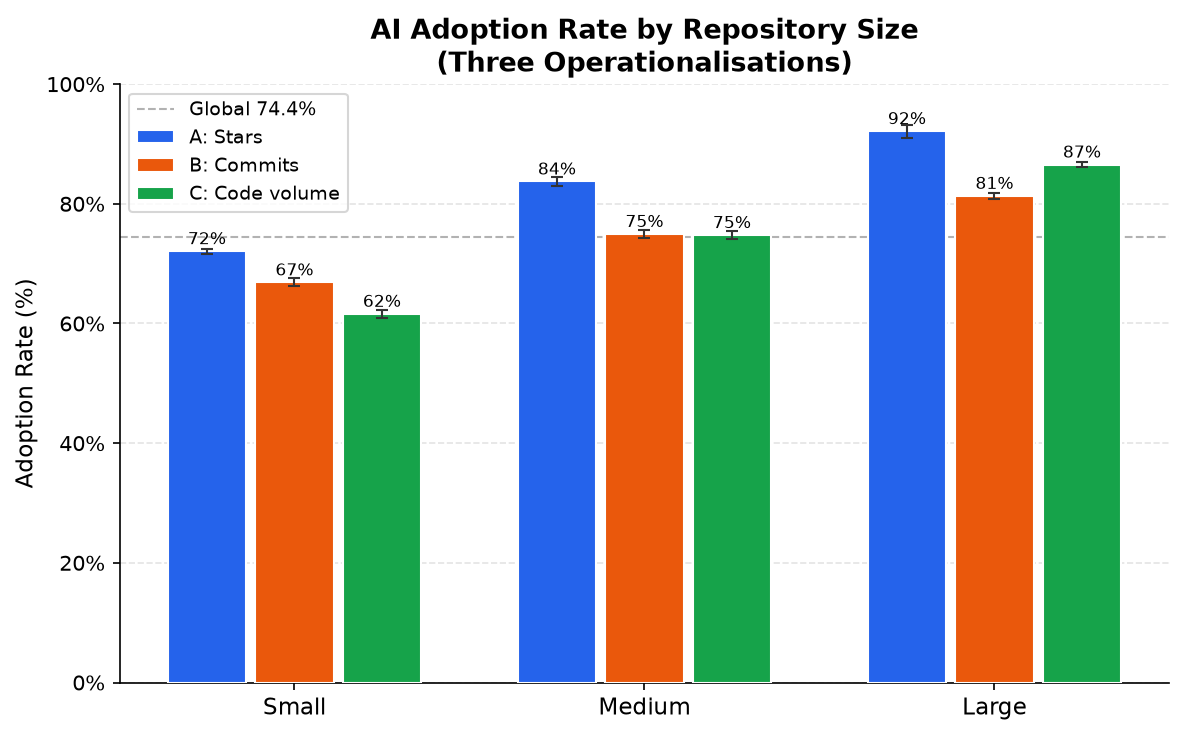
\includegraphics[width=0.78\textwidth]{fig_size_grouped_bar.png}\\
  \small\textit{Adoption rate by repository size (stars, commits, code volume)}
\end{center}

\vspace{6pt}
\hrule
\vspace{6pt}

% ─── MENA ─────────────────────────────────────────────────────────────────────
\section*{MENA Regional Analysis}

\textbf{Coverage:} 1,587 repos (2.6\% corpus, 4.7\% of located repos),
19 countries defined, 9 eligible ($\geq$30 repos).\\
\textbf{Overall MENA: 65.9\%} [63.5\%, 68.1\%] ---
below global 74.4\%.
Fisher exact vs global: $p = 1.38 \times 10^{-14}$ (significant).

\begin{multicols}{2}

\textbf{Sub-region breakdown:}

\begin{tabular}{@{}lrrr@{}}
\toprule
Sub-region & Repos & Rate\% & 95\% CI \\
\midrule
Gulf (UAE, SA, \ldots)  & 181 & 87.9* & [82.3, 91.8] \\
Levant (IL, JO, \ldots) & 238 & 81.9* & [76.6, 86.3] \\
Turkey                  & 509 & 72.1* & [68.1, 75.8] \\
North Africa            & 366 & 50.8* & [45.7, 55.9] \\
Iran                    & 293 & 47.1* & [41.5, 52.8] \\
\bottomrule
\end{tabular}

\columnbreak

\textbf{Eligible countries (9 of 19):}

\begin{tabular}{@{}lrr@{}}
\toprule
Country & Repos & Rate\% \\
\midrule
Saudi Arabia &  33 & 90.9* \\
UAE          & 119 & 87.4* \\
Israel       & 192 & 84.9* \\
Turkey       & 509 & 72.1* \\
Tunisia      &  59 & 55.9  \\
Egypt        & 176 & 55.1* \\
Algeria      &  49 & 49.0* \\
Iran         & 287 & 46.3* \\
Morocco      &  81 & 38.3* \\
\bottomrule
\end{tabular}

\end{multicols}

\vspace{4pt}
\begin{center}
  \begin{minipage}[t]{0.47\textwidth}
    \centering
    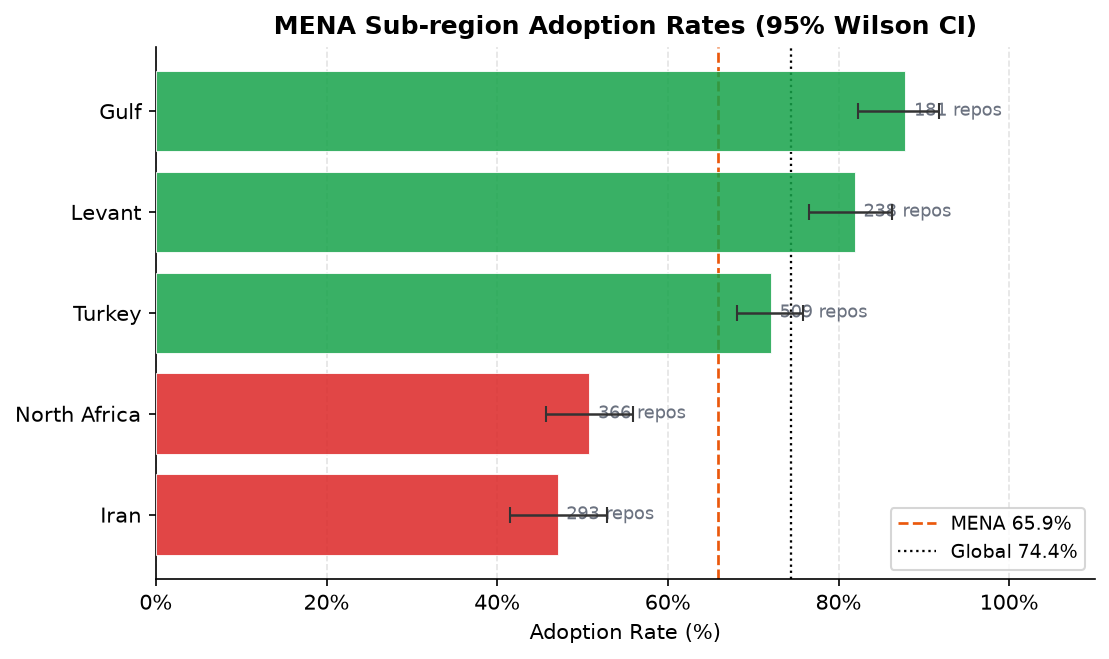
\includegraphics[width=\linewidth]{fig_mena_bar.png}\\
    \small\textit{MENA sub-region adoption rates with 95\% CIs}
  \end{minipage}
  \hfill
  \begin{minipage}[t]{0.47\textwidth}
    \centering
    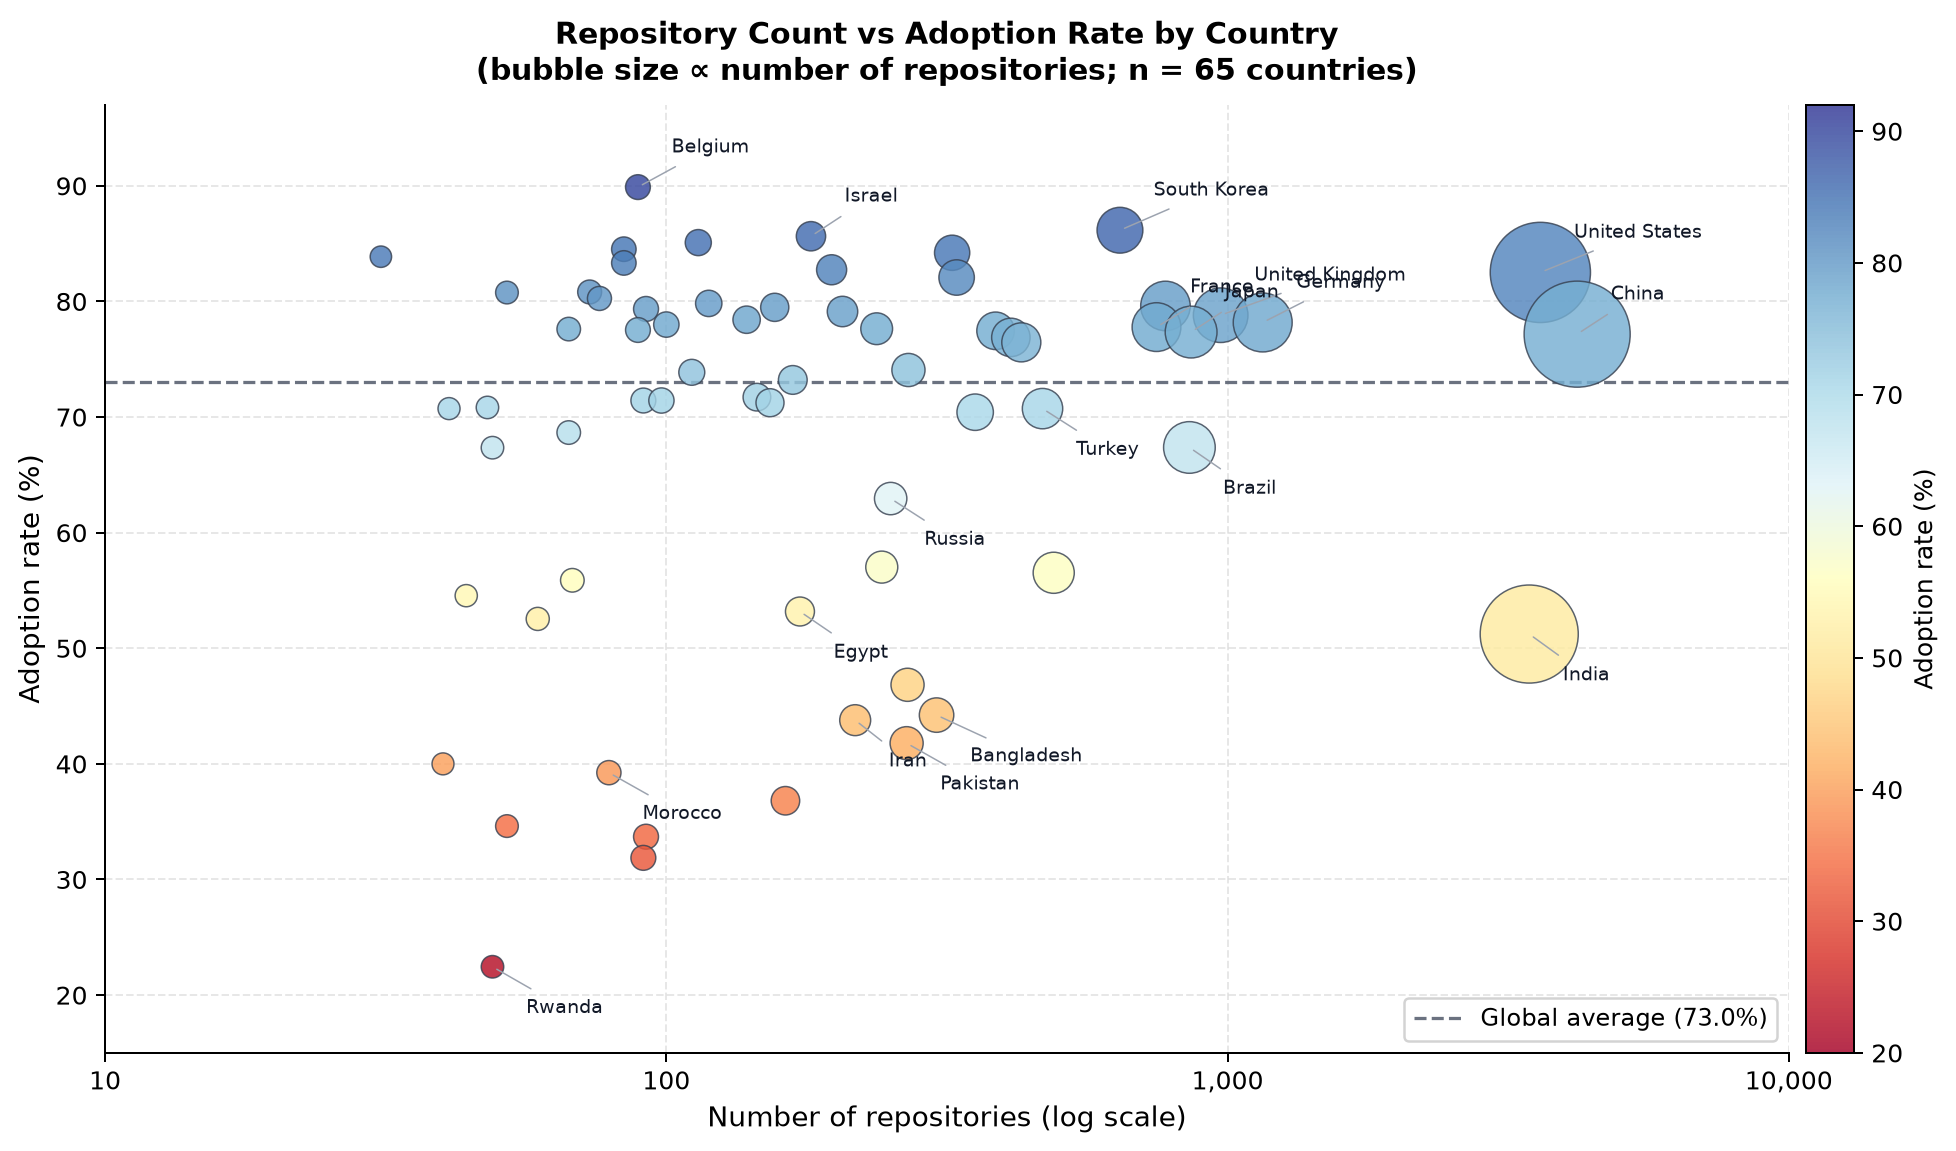
\includegraphics[width=\linewidth]{fig_country_bubble.png}\\
    \small\textit{Country bubble chart (size = $\sqrt{\text{repos}}$, position = adoption rate)}
  \end{minipage}
\end{center}

\vspace{6pt}
\hrule
\vspace{6pt}

% ─── RESEARCH QUESTIONS ───────────────────────────────────────────────────────
\section*{Research Questions --- Statistical Test Results}

\begin{tabular}{@{}p{3.2cm} p{5.5cm} p{3.2cm} p{3.0cm}@{}}
\toprule
\textbf{RQ} & \textbf{Finding} & \textbf{Test} & \textbf{Decision} \\
\midrule
\textbf{RQ1} Scope of adoption &
  74.4\% adoption rate (44,761/60,129). Wilson 95\% CI: [74.09\%, 74.79\%] &
  Binomial test vs $H_0{:}\ p \leq 5\%$ \newline $p = 0.00$ &
  \textcolor{red}{\textbf{Reject $H_0$}} \\[4pt]
\textbf{RQ2} Undercounting &
  Single-signal (Pass 3a): 47.2\%. Multi-signal: 74.4\%. Delta: \textbf{+27.21 pp}. $b=16{,}404$, $c=40$ &
  McNemar $\chi^2 = 16{,}282$ \newline $p = 0.00$ &
  \textcolor{red}{\textbf{Reject $H_0$}} \\[4pt]
\textbf{RQ3} Geographic variation &
  Rates range from 90.9\% (Saudi Arabia) to 27.5\% (Rwanda). 45/66 countries significantly differ from global mean &
  $\chi^2 = 2577.03$, $df=65$ \newline $p = 0.00$ &
  \textcolor{red}{\textbf{Reject $H_0$}} \\
\bottomrule
\end{tabular}

\vspace{6pt}
\renewcommand{\arraystretch}{1.4}
\noindent
\begin{tabular}{@{}
  >{\centering\arraybackslash\columncolor{red!15}}p{2.8cm}
  >{\columncolor{red!8}}p{14.0cm}@{}}
\textbf{RQ1 Reject $H_0$} &
  74.4\% adoption (44,761/60,129). Wilson 95\% CI: [74.09\%--74.79\%]. Binomial $p = 0.00$. \\
\textbf{RQ2 Reject $H_0$} &
  Multi-signal detects \textbf{+27.21\,pp} more than single-signal (47.2\% $\to$ 74.4\%). McNemar $\chi^2 = 16{,}282$, $p = 0.00$. \\
\textbf{RQ3 Reject $H_0$} &
  66-country range 27.5\%--90.9\%. 45/66 countries deviate significantly from global mean. $\chi^2 = 2577.03$, $p = 0.00$. \\
\end{tabular}
\renewcommand{\arraystretch}{1}

\vspace{6pt}
\hrule
\vspace{6pt}



\newpage
% ─── EXTENDED PIPELINE CHECK ──────────────────────────────────────────────────
\section*{Extended Pipeline Check --- Coverage Validation (Saturation Check)}

\textbf{Input:} 19,768 repos labelled \texttt{none} (15,368) or \texttt{ai\_assisted} (4,397) after Stage 3.\\
\textbf{Purpose:} Verify Stage 3 saturation by scanning for signals not included in the original three passes.

\vspace{4pt}
\begin{tabular}{@{}p{2.2cm} p{5.8cm} p{2.4cm} r r@{}}
\toprule
\textbf{Pass} & \textbf{What was checked} & \textbf{Signal (tier)} & \textbf{Input} & \textbf{New agentic} \\
\midrule
\textbf{5a} --- Extended bots &
  12 additional bot accounts as commit/PR authors:
  \textit{sweep-ai, openhands-agent, codegen-sh, amazon-q-developer,
  coderabbitai, junie, factory-bot, github-copilot,
  devin-ai-integration, jules-google, ellipsis-dev, greptileai} &
  bot\_author (STRONG) & 19,768 & \textbf{0} \\[6pt]
\textbf{5b} --- Workflow scan &
  11 AI GitHub Actions in \texttt{.github/workflows/} YAML content:
  \textit{anthropic/claude-code-action, sweep-ai/sweep,
  All-Hands-AI/OpenHands, codegen-sh/codegen, devin-ai-integration/devin,
  junie-jetbrains/junie, amazon-q-developer-action,
  greptileai/greptile-action, ellipsis-dev/ellipsis-action,
  factory-ai/factory-action, github/copilot-autofix-action} &
  ci\_ai\_action (STRONG) & 19,768 & \textbf{0} \\[6pt]
\textbf{5c} --- Extended configs &
  18 config paths/dirs not in Stage 3:
  \texttt{.amazonq/}, \texttt{.continue/}, \texttt{.codeium/},
  \texttt{sweep.yaml}, \texttt{coderabbit.yaml}, \texttt{.cursorrules},
  \texttt{.cursor/}, \texttt{.mentat/}, \texttt{.sourcegraph/},
  \texttt{.ellipsis.yaml}, \texttt{.tabnine/} and others &
  config\_file (MEDIUM) & 19,768 & \textbf{0} \\
\bottomrule
\end{tabular}

\vspace{4pt}
\textbf{Conclusion:} Zero new detections across all three extended passes confirms that Stage 3's signal set
has reached \textbf{saturation}. The remaining 19,768 repos show no detectable agentic footprint using any
publicly observable signal. Silent IDE usage (e.g.\ Cursor, Copilot inline completions with no config file)
remains undetectable by design and is documented as a validity threat.

\vspace{6pt}
\noindent
\colorbox{green!15}{\parbox{0.975\linewidth}{
\vspace{3pt}
\centering
\renewcommand{\arraystretch}{1.25}
\begin{tabular}{@{}
  >{\centering\arraybackslash\columncolor{green!25}}p{3.8cm}
  >{\centering\arraybackslash\columncolor{green!25}}p{3.8cm}
  >{\centering\arraybackslash\columncolor{green!25}}p{3.8cm}
  >{\centering\arraybackslash\columncolor{green!10}}p{4.4cm}@{}}
\textbf{5a Extended bots} & \textbf{5b Workflows} & \textbf{5c Configs} & \textbf{Verdict} \\
12 new bot accounts & 11 new AI actions & 18 new config paths & \\
\textbf{0 new agentic} & \textbf{0 new agentic} & \textbf{0 new agentic} &
\textbf{Stage 3 = saturated} \\
\end{tabular}
\renewcommand{\arraystretch}{1}
\vspace{3pt}
}}

\vspace{6pt}
\hrule
\vspace{6pt}

\newpage
% ─── FRAMEWORK ANALYSIS ───────────────────────────────────────────────────────
\section*{AI Adoption by Framework \& Package Ecosystem}

\textbf{Note:} Frameworks are multi-label per repo (e.g.\ React + Electron counts in both rows),
so framework rows are not mutually exclusive partitions of the corpus.

\vspace{4pt}
\textbf{Top 20 frameworks} by repo count:

\vspace{3pt}
\begin{tabular}{@{}lrrrr@{}}
\toprule
Framework & Repos & Agentic\% & AI-assist\% & No AI\% \\
\midrule
React          & 30,614 & 65.2 & 7.1 & 27.7 \\
Next.js        & 10,807 & 63.6 & 6.8 & 29.6 \\
Express        &  7,131 & 57.8 & 7.1 & 35.1 \\
Electron       &  4,366 & 75.6 & 8.2 & 16.2 \\
Tauri          &  2,777 & 73.4 & 9.2 & 17.5 \\
Hono           &  2,672 & 82.1 & 6.6 & 11.2 \\
Vue            &  1,911 & 68.3 & 8.1 & 23.6 \\
Astro          &  1,417 & 83.5 & 6.5 & 10.0 \\
React Native   &  1,387 & 67.6 & 7.2 & 25.2 \\
Fastify        &  1,339 & 77.3 & 8.4 & 14.3 \\
Expo           &  1,110 & 69.0 & 5.9 & 25.1 \\
Svelte         &  1,076 & 74.9 & 8.4 & 16.7 \\
NestJS         &    933 & 62.0 & 8.4 & 29.7 \\
VitePress      &    923 & 77.8 & 6.5 & 15.7 \\
TanStack Start &    670 & 79.4 & 4.5 & 16.1 \\
Capacitor      &    588 & 68.2 & 7.1 & 24.7 \\
Solid          &    573 & 77.8 & 8.0 & 14.1 \\
SvelteKit      &    544 & 75.6 & 9.0 & 15.4 \\
tRPC           &    528 & 70.3 & 7.6 & 22.2 \\
Preact         &    472 & 74.2 & 7.0 & 18.9 \\
\bottomrule
\end{tabular}

\vspace{6pt}
\textbf{Highest agentic adoption:} Astro 83.5\%, Hono 82.1\%, TanStack Start 79.4\%, VitePress + Solid 77.8\%\\
\textbf{Lowest agentic adoption:} Express 57.8\%, NestJS 62.0\%, Next.js 63.6\%\\
\textbf{Largest corpus:} React (30,614 repos, 65.2\%) --- over half the entire corpus uses React.

\vspace{6pt}
\textbf{Framework combinations} (React paired, mutually exclusive; 965 repos using all three excluded):

\vspace{3pt}
\begin{tabular}{@{}lrrrr@{}}
\toprule
Combination & Repos & Agentic\% & AI-assist\% & No AI\% \\
\midrule
React + Next.js (no Express) & 9,799 & 66.4 & 6.8 & 26.9 \\
React + Express (no Next.js) & 3,392 & 56.0 & 6.9 & 37.1 \\
\bottomrule
\end{tabular}

\vspace{6pt}
\textbf{AI adoption by package ecosystem:}

\vspace{3pt}
\begin{tabular}{@{}lrrrr@{}}
\toprule
Ecosystem & Repos & Agentic\% & AI-assist\% & No AI\% \\
\midrule
pnpm          & 12,229 & 77.0 & 7.0 & 16.0 \\
deno          &    250 & 76.0 & 4.8 & 19.2 \\
npm\_no\_lock &  7,979 & 71.8 & 6.6 & 21.6 \\
npm           & 28,248 & 67.8 & 7.5 & 24.7 \\
bun           &    107 & 62.6 & 3.7 & 33.6 \\
yarn          &  1,091 & 57.2 & 6.7 & 36.1 \\
vanilla       & 10,177 & 50.9 & 7.9 & 41.1 \\
\bottomrule
\end{tabular}

\vspace{4pt}
{\small pnpm (77.0\%) and deno (76.0\%) show highest agentic adoption; vanilla (50.9\%) and yarn (57.2\%) lowest.
pnpm's higher rate likely reflects modern toolchain projects where AI agent setup is more common.
vanilla repos (no lockfile) skew older or simpler projects with less AI tooling.}

\vspace{4pt}
\begin{center}
  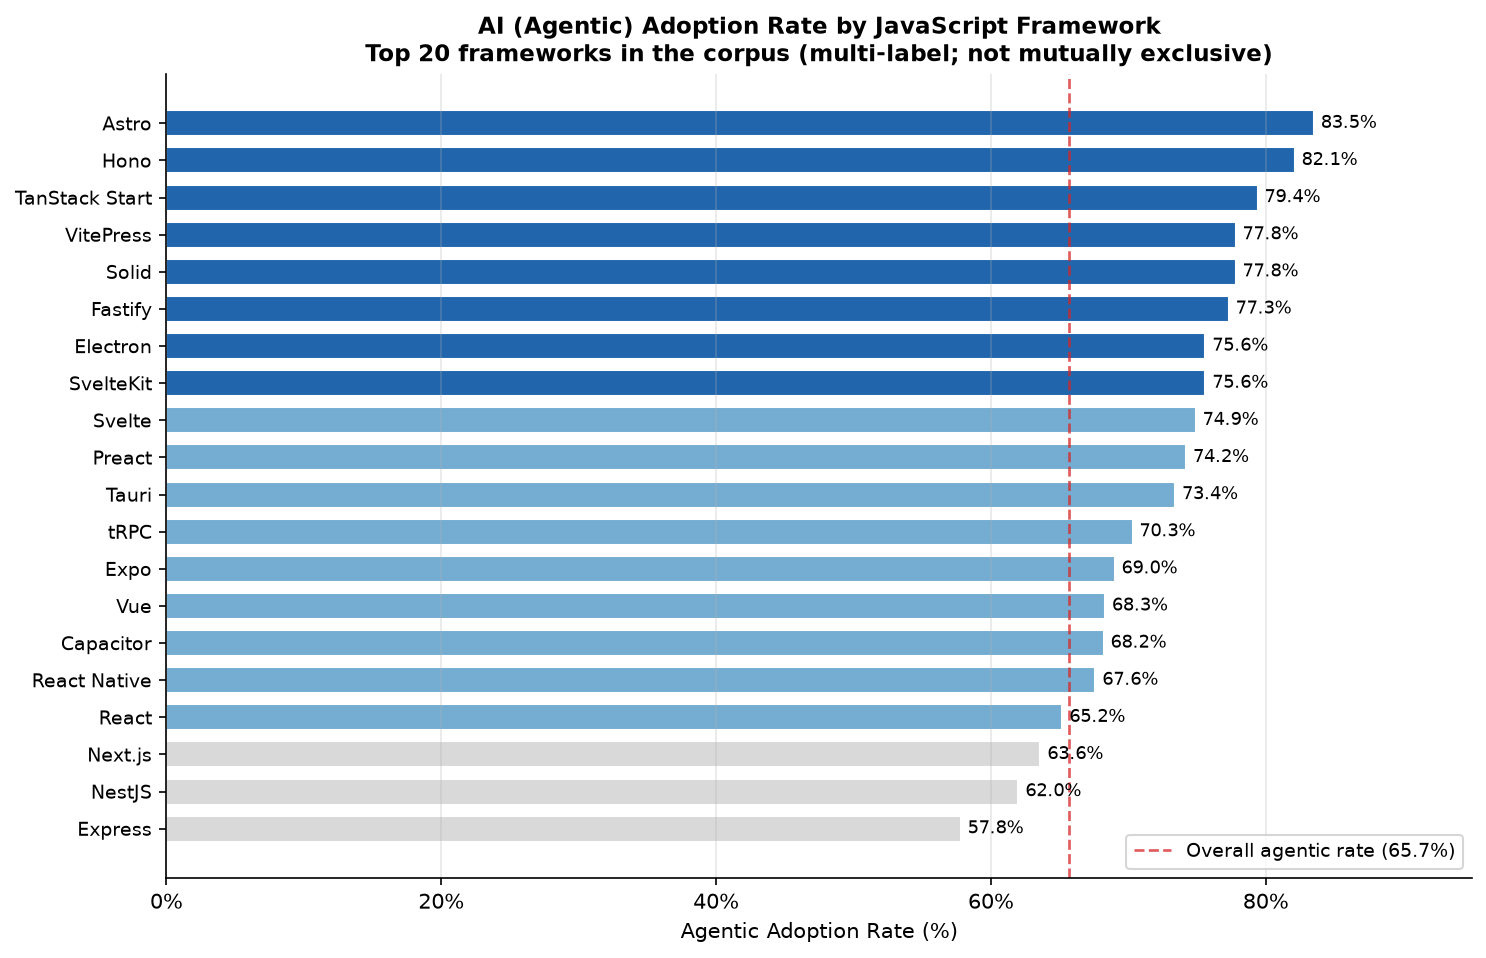
\includegraphics[width=0.82\textwidth]{fig_framework_adoption.png}\\
  \small\textit{Agentic adoption rate for top 20 JS frameworks (dashed line = overall 67.1\%)}
\end{center}

\vspace{6pt}
\hrule
\vspace{6pt}

\newpage
% ─── PRICING ANALYSIS ─────────────────────────────────────────────────────────
\section*{AI Tool Pricing vs Country Income --- Adoption Analysis}

\textbf{Hypothesis:} Does tool pricing (paid vs free) explain lower adoption rates in lower-income countries?

\vspace{6pt}
\begin{multicols}{2}

\textbf{Tool pricing classification:}

\begin{tabular}{@{}lll@{}}
\toprule
Tool & Pricing & Category \\
\midrule
Claude Code       & Pro \$20/mo required  & Paid \\
OpenAI Codex CLI  & API credits required  & Paid \\
Devin             & \$500+/mo             & Paid \\
Junie             & JetBrains sub.        & Paid \\
Codegen           & Paid only             & Paid \\
Factory           & Paid only             & Paid \\
Greptile          & Paid only             & Paid \\
Ellipsis          & Paid (OSS free)       & Paid \\
\midrule
GitHub Copilot    & Free tier + student   & Free \\
Cursor            & Free tier + student   & Free \\
OpenHands         & OSS / self-host       & Free \\
Gemini CLI        & Free tier             & Free \\
Amazon Q          & Free tier + edu       & Free \\
Sweep AI          & Free for public repos & Free \\
CodeRabbit        & Free for public repos & Free \\
Windsurf          & Free tier             & Free \\
Aider             & OSS, free             & Free \\
Jules             & Free (Google preview) & Free \\
\bottomrule
\end{tabular}

\columnbreak

\textbf{World Bank income groups (2024):}

\begin{tabular}{@{}ll@{}}
\toprule
Group & Countries in corpus \\
\midrule
\textbf{HIC} & US, UK, Germany, France, Japan, \\
High Income  & South Korea, Australia, Canada, \\
             & Israel, UAE, Sweden, Switzerland, \\
             & Netherlands, Denmark, Singapore, \\
             & Taiwan, Belgium, Norway, Austria, \\
             & Finland, NZ, Ireland, Hong Kong, \\
             & Italy, Spain, Portugal, Czech Rep. \\[4pt]
\textbf{UMIC} & China, Brazil, Turkey, Russia, \\
Upper-Middle  & Mexico, Argentina, Thailand, \\
              & Malaysia, Colombia, Ukraine, \\
              & South Africa, Poland, Romania, \\
              & Bulgaria, Serbia, Chile, Egypt, \\
              & Georgia, Kazakhstan, Uzbekistan, \\
              & Algeria, Tunisia, Hungary, Peru \\[4pt]
\textbf{LMIC} & India, Vietnam, Philippines, \\
Lower-Middle  & Indonesia, Bangladesh, Pakistan, \\
              & Nigeria, Ghana, Kenya, Morocco, \\
              & Sri Lanka, Nepal, Ethiopia, Iran \\[4pt]
\textbf{LIC}  & Rwanda \\
Low Income    & \\
\bottomrule
\end{tabular}

\end{multicols}

\vspace{6pt}
\textbf{Results by income group} (33,848 located repos):

\vspace{3pt}
\begin{tabular}{@{}lrrrrrr@{}}
\toprule
Income Group & Repos & Adoption\% & Agentic & Paid tool\% & Free tool\% \\
\midrule
High Income        & 15,020 & 81.3 & 11,193 & 72.6 & 11.4 \\
Upper-Middle Inc.  & 10,534 & 74.6 &  6,946 & 64.0 & 11.0 \\
Lower-Middle Inc.  &  7,697 & 52.4 &  3,490 & 60.8 & 24.3 \\
Low Income         &     51 & 27.5 &     12 & 50.0 & 41.7 \\
\bottomrule
\end{tabular}

\vspace{4pt}
\begin{center}
  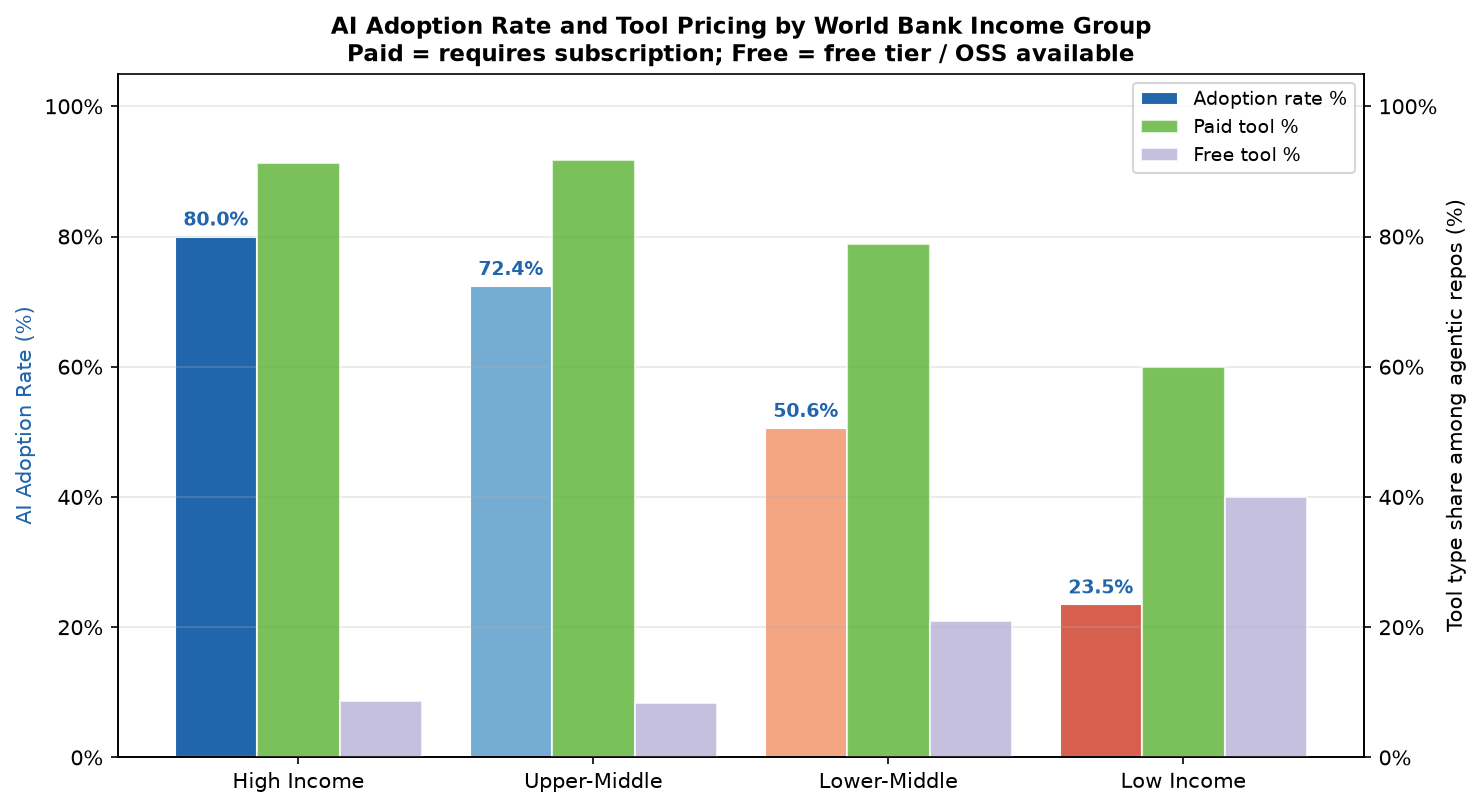
\includegraphics[width=0.82\textwidth]{fig_pricing_income.png}\\
  \small\textit{Adoption rate (left axis) and tool-type share (right axis) by income group}
\end{center}

\newpage
% ─── EXTENDED ANALYSIS ────────────────────────────────────────────────────────
\section*{Extended Analysis}
\begin{multicols}{2}
\footnotesize

% ── E1: Time Series ───────────────────────────────────────────────────────────
\subsection*{AI Adoption Over Time}
\textbf{Range:} Feb 2025 -- Sep 2026 (20 months, 60,129 repos).

\vspace{2pt}
\begin{tabular}{@{}lrrr@{}}
\toprule
Month & Repos & Adopt\% & Agentic\% \\
\midrule
2025-02 &    299 & 50.5 & 44.5 \\
2025-03 &  1,862 & 53.1 & 46.1 \\
2025-04 &  1,713 & 53.7 & 47.6 \\
2025-05 &  1,755 & 54.0 & 48.5 \\
2025-06 &  1,966 & 60.5 & 54.1 \\
2025-07 &  2,082 & 60.6 & 54.1 \\
2025-08 &  2,098 & 63.4 & 56.8 \\
2025-09 &  2,101 & 59.3 & 52.8 \\
2025-10 &  2,386 & 64.7 & 58.4 \\
2025-11 &  2,391 & 68.9 & 62.1 \\
2025-12 &  2,905 & 71.7 & 64.3 \\
2026-01 &  3,871 & 77.7 & 70.7 \\
2026-02 &  5,184 & 82.8 & 76.4 \\
2026-03 &  5,993 & 84.3 & 76.7 \\
2026-04 &  4,808 & 84.0 & 76.5 \\
2026-05 &  4,429 & 82.9 & 74.6 \\
2026-06 &  4,207 & 80.9 & 72.8 \\
2026-07 &  4,044 & 82.0 & 73.8 \\
2026-08 &  3,867 & 77.3 & 68.4 \\
2026-09 &  2,079 & 77.6 & 69.0 \\
\bottomrule
\end{tabular}

\vspace{3pt}
\textbf{Key findings:}
\begin{itemize}\setlength\itemsep{0pt}
  \item Adoption rose from \textbf{50.5\%} (Feb 2025)
        to peak \textbf{84.3\%} (Mar 2026).
  \item Sharpest growth: Dec 2025 $\to$ Feb 2026
        (+11\,pp in 2 months).
  \item Plateau at $\approx$82--84\% from Feb--May 2026.
\end{itemize}

\vspace{3pt}
\hrule
\vspace{3pt}

% ── E2: Size Comparison ───────────────────────────────────────────────────────
\subsection*{Repo Size by Adoption Category}
Kruskal-Wallis (3-way) + Mann-Whitney U (Agentic vs No AI).

\vspace{2pt}
\begin{tabular}{@{}lrrr@{}}
\toprule
Metric & No AI & AI-Asst & Agentic \\
       & (med.)& (med.)  & (med.)  \\
\midrule
Commits   & 134 & 162 & 200 \\
Code (KB) & 495 & 802 & 1{,}021 \\
\midrule
Stars     &   7 &  11 &   11 \\
Forks     &   1 &   2 &    2 \\
\bottomrule
\end{tabular}

\vspace{2pt}
\textit{All MW $p < 10^{-300}$;\;
Commits and code volume both increase monotonically across adoption groups.}

\columnbreak

% ── E3: React + Next.js Subset ────────────────────────────────────────────────
\subsection*{React + Next.js Subset (9,799 repos)}

\textbf{Adoption summary:}

\vspace{2pt}
\begin{tabular}{@{}lrr@{}}
\toprule
Category & Count & \% \\
\midrule
Agentic         & 6,505 & 66.4 \\
AI-Assisted     &   663 &  6.8 \\
No AI           & 2,631 & 26.9 \\
\midrule
\textbf{Adopted}& \textbf{7,168} & \textbf{73.2} \\
\bottomrule
\end{tabular}

\vspace{4pt}
\textbf{Top agents (agentic repos):}

\vspace{2pt}
\begin{tabular}{@{}lrr@{}}
\toprule
Agent & Count & \% agentic \\
\midrule
Claude Code     & 4,507 & 69.3 \\
Generic         & 2,864 & 44.0 \\
Cursor          &   855 & 13.1 \\
GitHub Copilot  &   670 & 10.3 \\
OpenAI Codex    &   369 &  5.7 \\
CodeRabbit      &   144 &  2.2 \\
\bottomrule
\end{tabular}

\vspace{4pt}
\textbf{Country ranking ($\geq$30 repos):}

\vspace{2pt}
\begin{tabular}{@{}clrr@{}}
\toprule
\# & Country & $n$ & Adopt\% \\
\midrule
 1 & Colombia      &  30 & 83.3 \\
 2 & South Korea   & 108 & 83.3 \\
 3 & Australia     & 103 & 82.5 \\
 4 & Portugal      &  33 & 81.8 \\
 5 & Netherlands   &  43 & 81.4 \\
 6 & Italy         &  58 & 81.0 \\
 7 & United States & 772 & 80.1 \\
 8 & China         & 717 & 79.5 \\
 9 & Germany       & 136 & 78.7 \\
10 & Spain         &  65 & 78.5 \\
\bottomrule
\end{tabular}

\vspace{4pt}
\textbf{Key findings:}
\begin{itemize}\setlength\itemsep{0pt}
  \item Overall adoption (73.2\%) is slightly below the full corpus (74.4\%).
  \item Claude Code takes \textbf{69.3\%} of agent detections in this
        subset; Generic (44.0\%) is unusually high, reflecting many
        multi-agent repos.
  \item Colombia and South Korea lead; US (\#7) and China (\#8) rank
        lower than in the full corpus.
\end{itemize}

\end{multicols}

\vspace{4pt}
\begin{center}
  \begin{minipage}[t]{0.47\textwidth}
    \centering
    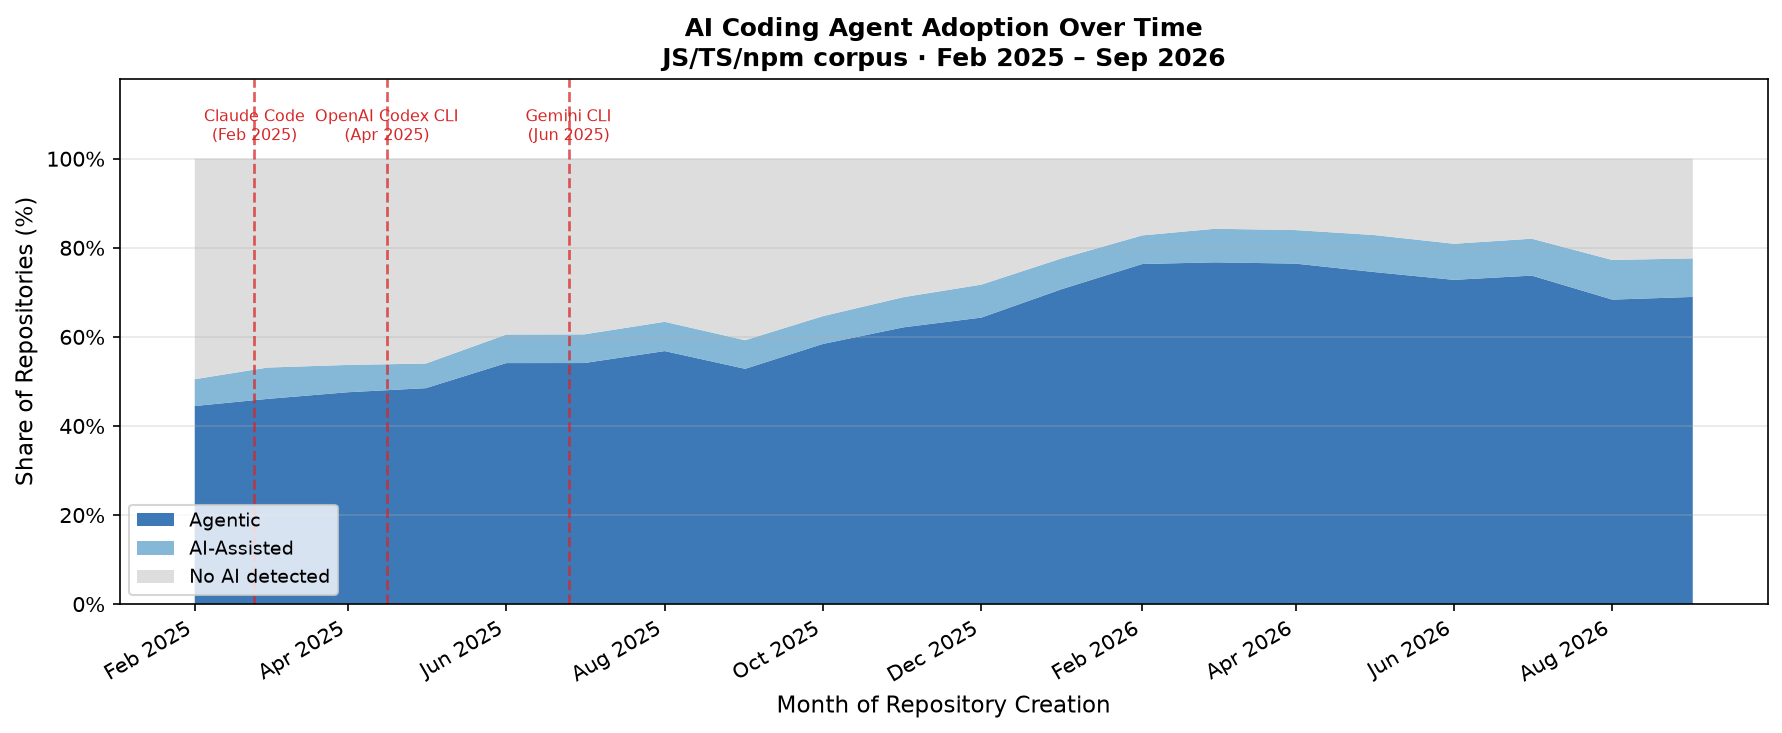
\includegraphics[width=\linewidth]{stage5/fig_adoption_time_series.png}\\
    \small\textit{E1 --- Monthly adoption rate (stacked, with release milestones)}
  \end{minipage}
  \hfill
  \begin{minipage}[t]{0.47\textwidth}
    \centering
    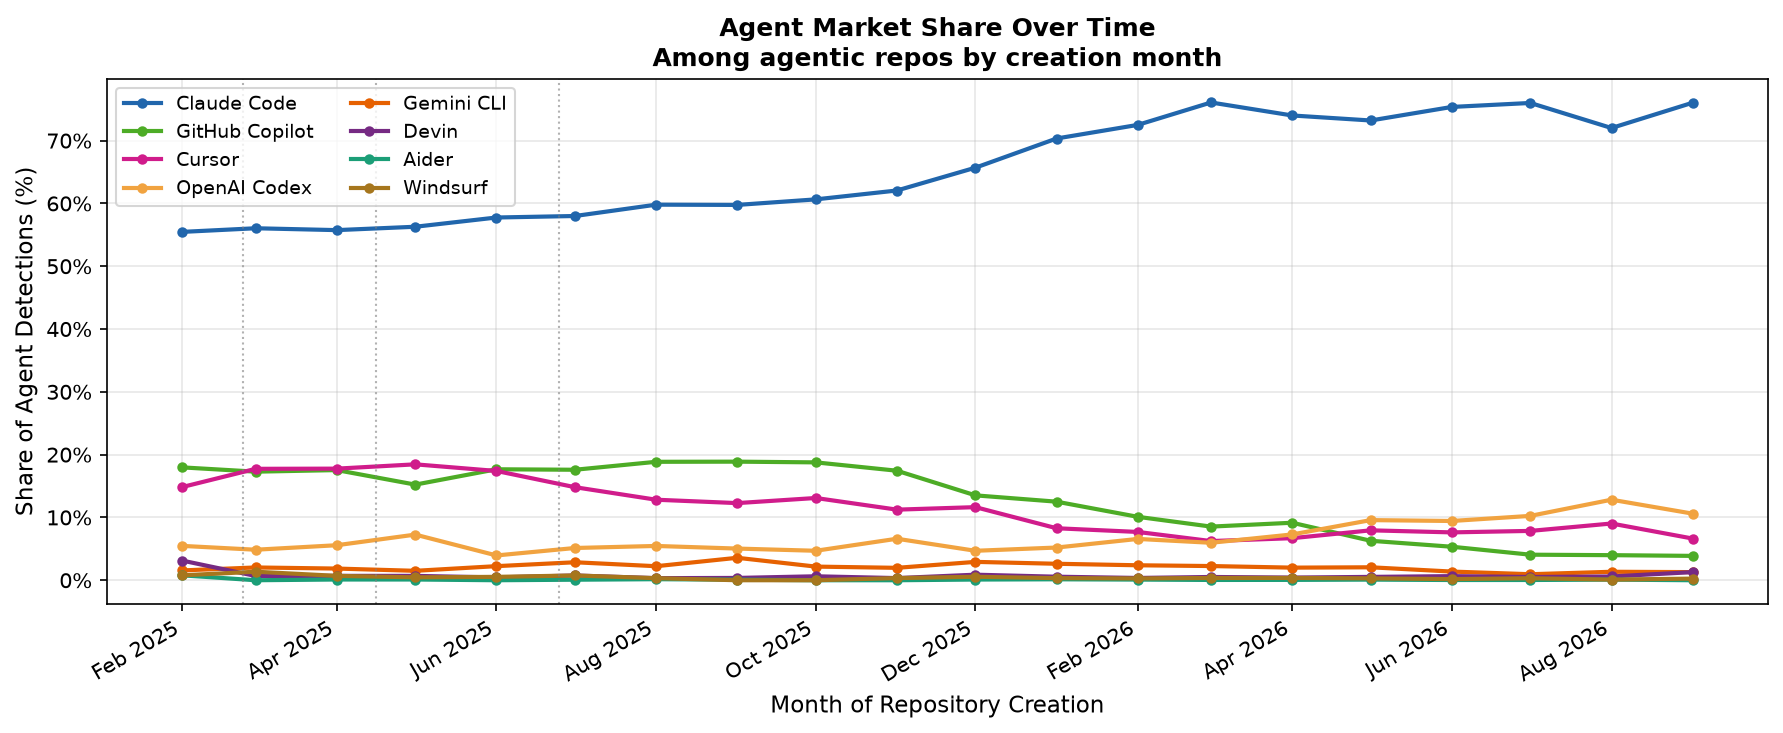
\includegraphics[width=\linewidth]{stage5/fig_agent_market_share.png}\\
    \small\textit{E1 --- Agent market share over time}
  \end{minipage}
\end{center}

\vspace{4pt}
\begin{center}
  \begin{minipage}[t]{0.47\textwidth}
    \centering
    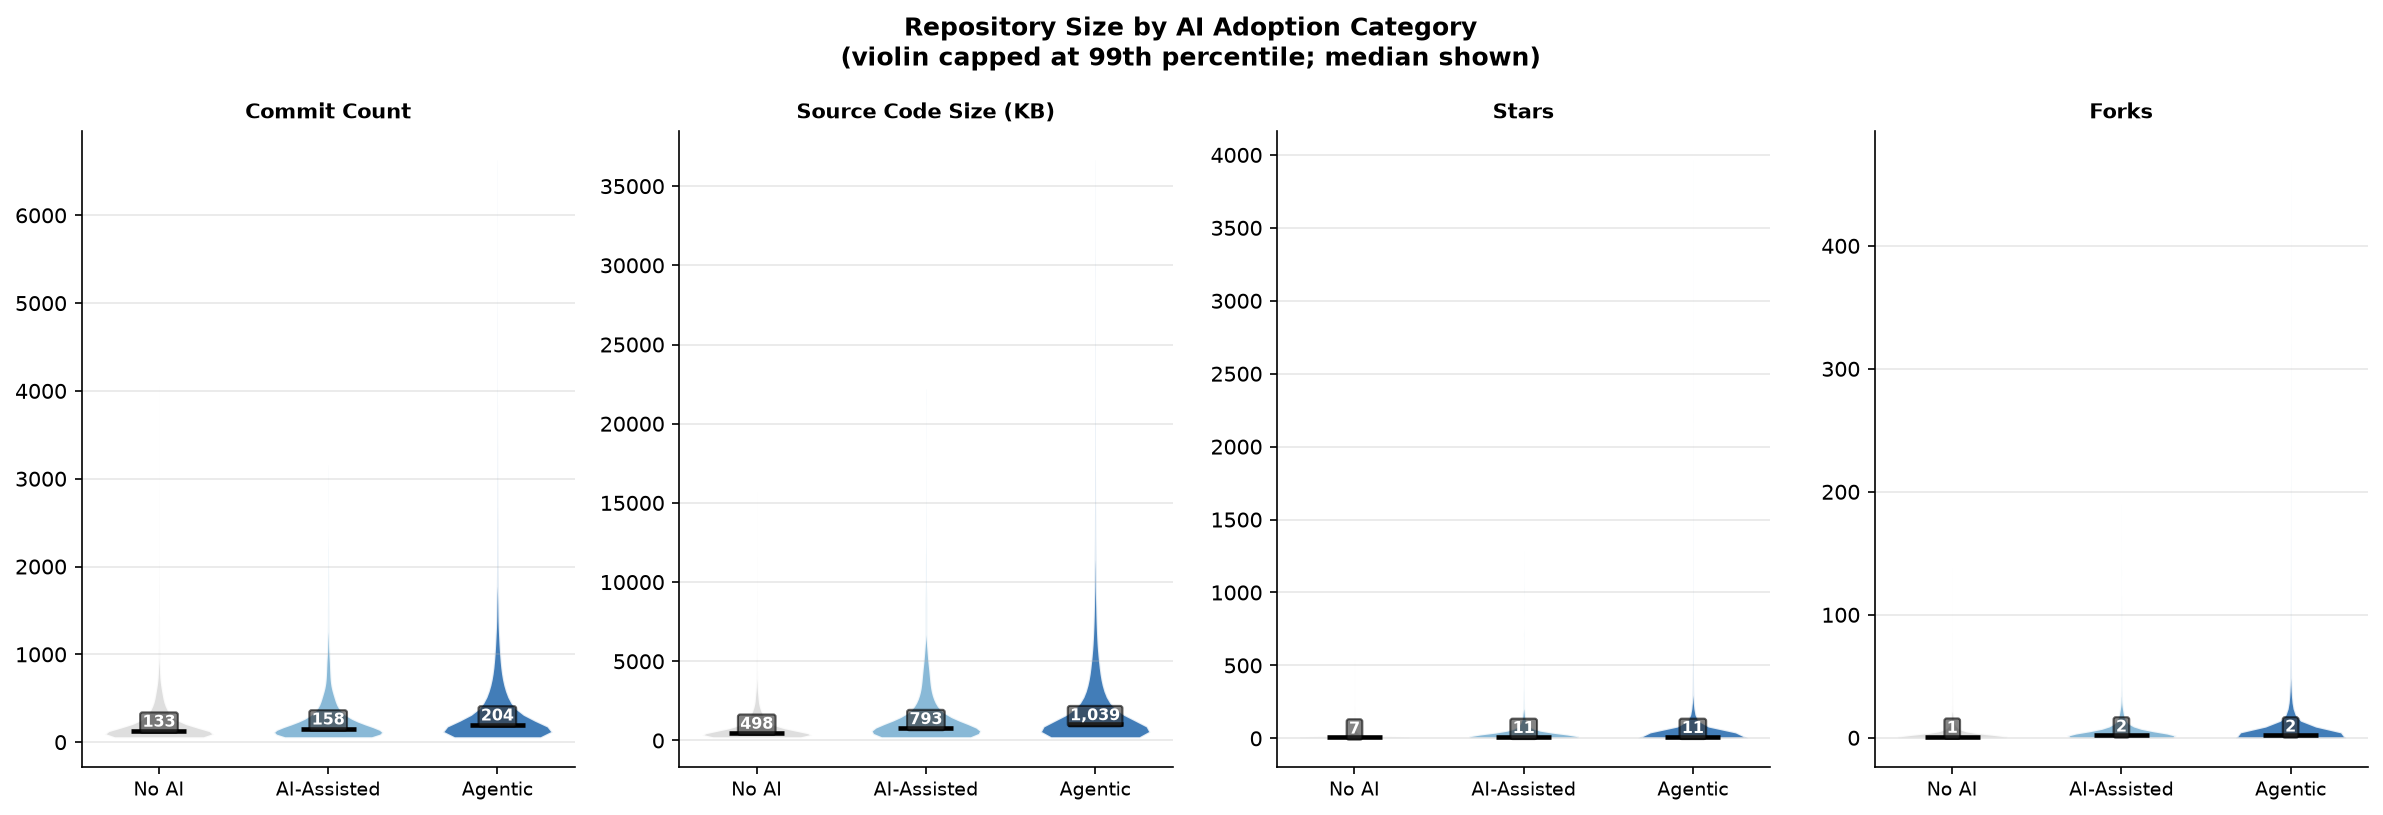
\includegraphics[width=\linewidth]{stage5/fig_size_comparison.png}\\
    \small\textit{E2 --- Repo size violin plots by adoption group (99th-pct cap)}
  \end{minipage}
  \hfill
  \begin{minipage}[t]{0.47\textwidth}
    \centering
    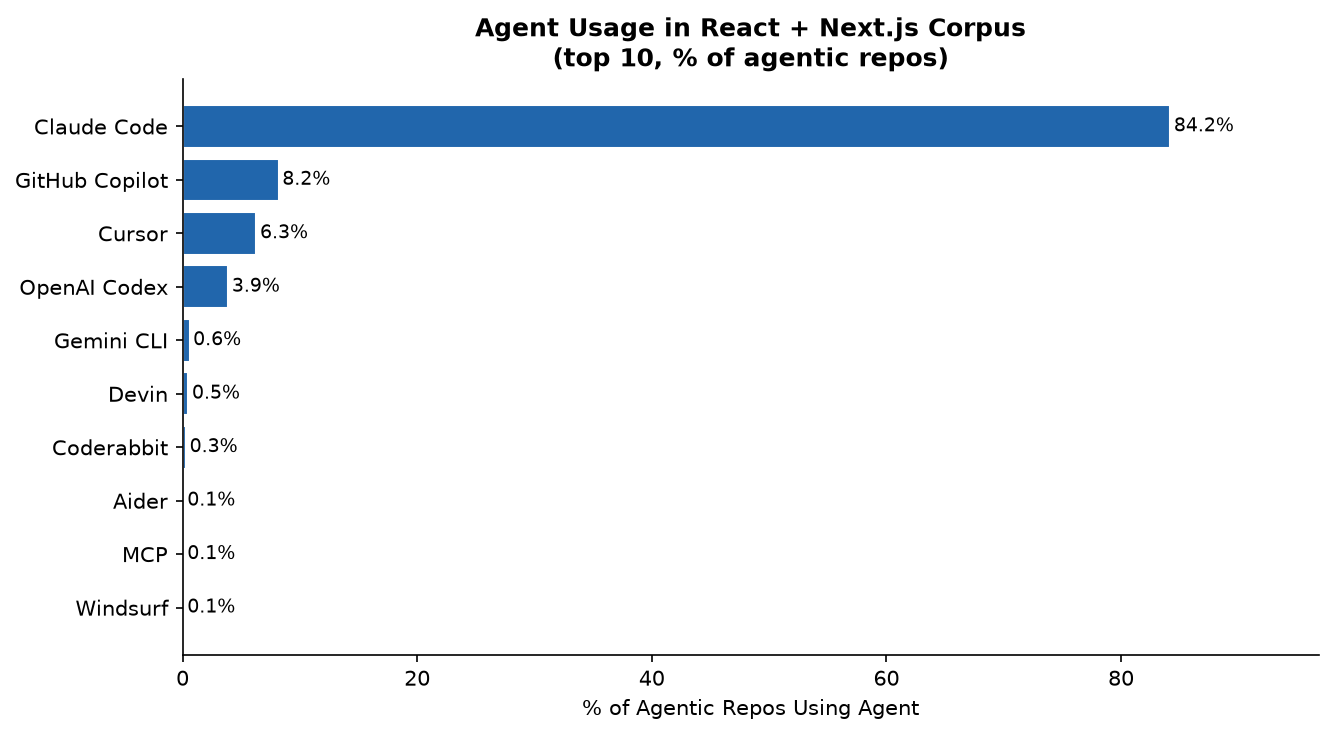
\includegraphics[width=\linewidth]{stage5/fig_rn_agent_breakdown.png}\\
    \small\textit{E3 --- Agent usage in React + Next.js agentic repos}
  \end{minipage}
\end{center}

\vspace{4pt}
\begin{center}
  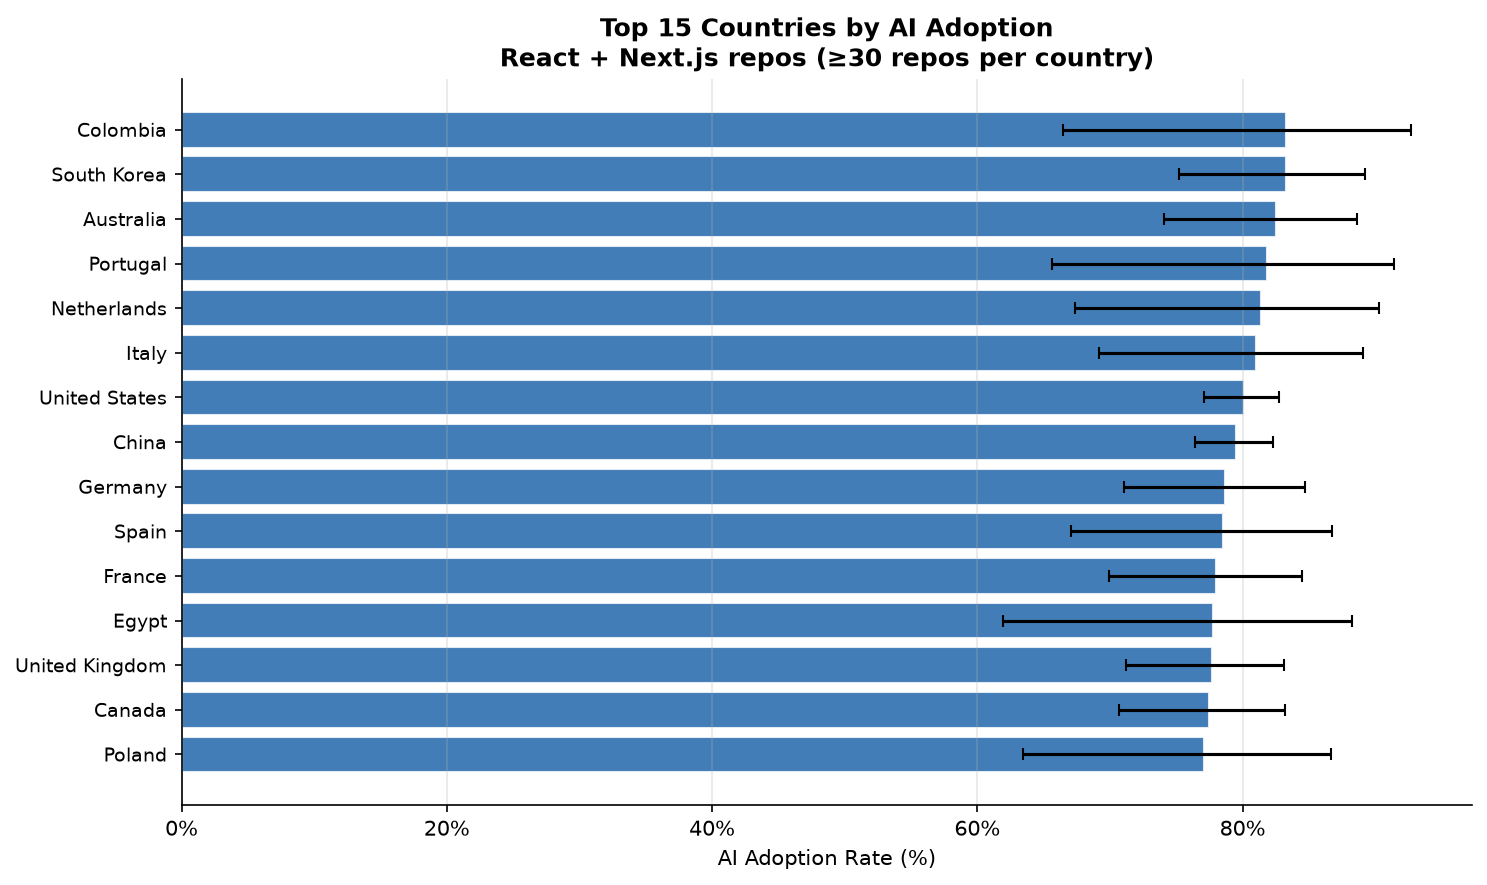
\includegraphics[width=0.60\textwidth]{stage5/fig_rn_country_ranking.png}\\
  \small\textit{E3 --- Top 15 countries by AI adoption in the React + Next.js subset}
\end{center}

\vspace{4pt}
\hrule
\vspace{4pt}

% ── E4: First Agent Commit + Adoption Patterns ───────────────────────────────
\begin{multicols}{2}
\footnotesize

\subsection*{First Claude Code Commit \& Adoption Patterns}
\textbf{Population:} 1,137 sampled Claude Code agentic repos (trailer\_count $> 0$).\\
Trailers found in \textbf{1,088/1,137 repos (95.7\%)}.

\vspace{3pt}
\textbf{Trailer timing (days from repo creation to first AI commit):}

\vspace{2pt}
\begin{tabular}{@{}lrr@{}}
\toprule
Timing & Count & \% \\
\midrule
Day 1 ($\leq$7\,d)  & 453 & 41.6 \\
Early (8--30\,d)    & 139 & 12.8 \\
Late ($>$30\,d)     & 496 & 45.6 \\
Not found           &  49 &  4.3 \\
\bottomrule
\end{tabular}

\vspace{2pt}
Median days to first trailer: \textbf{18.5\,d}.\quad
Median commits before AI: \textbf{28.1\%}.

\columnbreak

\textbf{Adoption patterns:}

\vspace{2pt}
\begin{tabular}{@{}lrr@{}}
\toprule
Pattern & Count & \% \\
\midrule
Trailer-only (no config)        &   946 & 83.2 \\
AI-native (config + trailer $\leq$7d) &  63 &  5.5 \\
Config-first                    &    56 &  4.9 \\
Trailer-first                   &    23 &  2.0 \\
Not found                       &    49 &  4.3 \\
\bottomrule
\end{tabular}

\vspace{2pt}
Config files found in \textbf{148/1,137 repos (13.0\%)}.\;
Median config day: \textbf{2\,d}.

\vspace{3pt}
\textbf{Key findings:}
\begin{itemize}\setlength\itemsep{0pt}
  \item Most developers (\textbf{83.2\%}) use Claude Code without ever
        committing a config file.
  \item The bimodal timing split (41.6\% day-1 vs 45.6\% late) suggests two
        archetypes: \emph{AI-native} starters vs developers who adopt
        Claude Code mid-project.
  \item When a config file is present, it typically appears very early
        (median day 2).
  \item Only 5.5\% of repos show the full AI-native pattern.
\end{itemize}

\end{multicols}

\vspace{4pt}
\begin{center}
  \begin{minipage}[t]{0.47\textwidth}
    \centering
    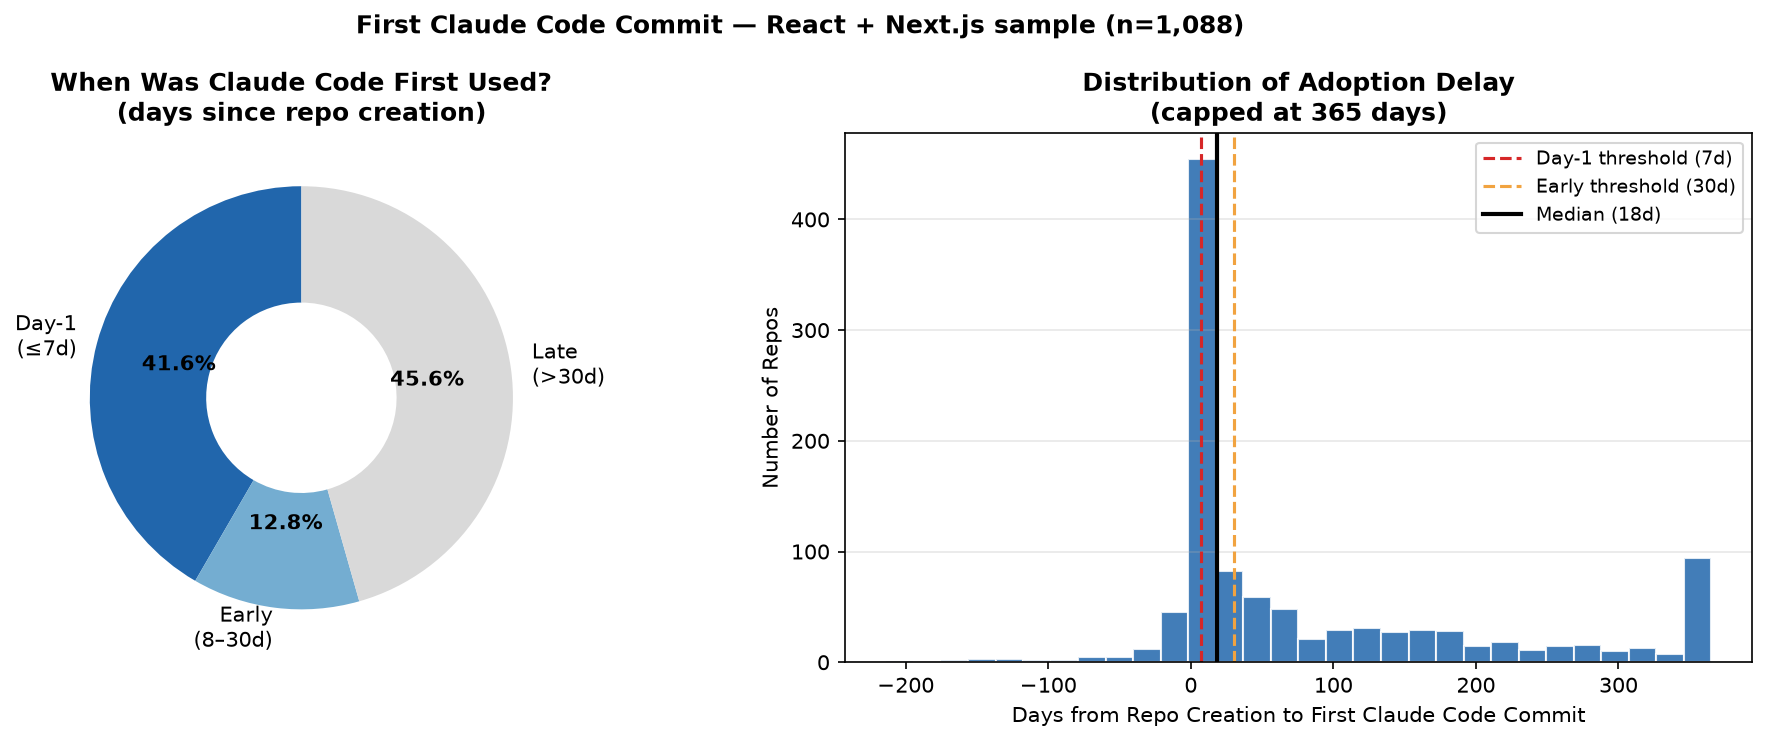
\includegraphics[width=\linewidth]{stage5/fig_adoption_timing.png}\\
    \small\textit{E4 --- First AI commit timing (donut + histogram)}
  \end{minipage}
  \hfill
  \begin{minipage}[t]{0.47\textwidth}
    \centering
    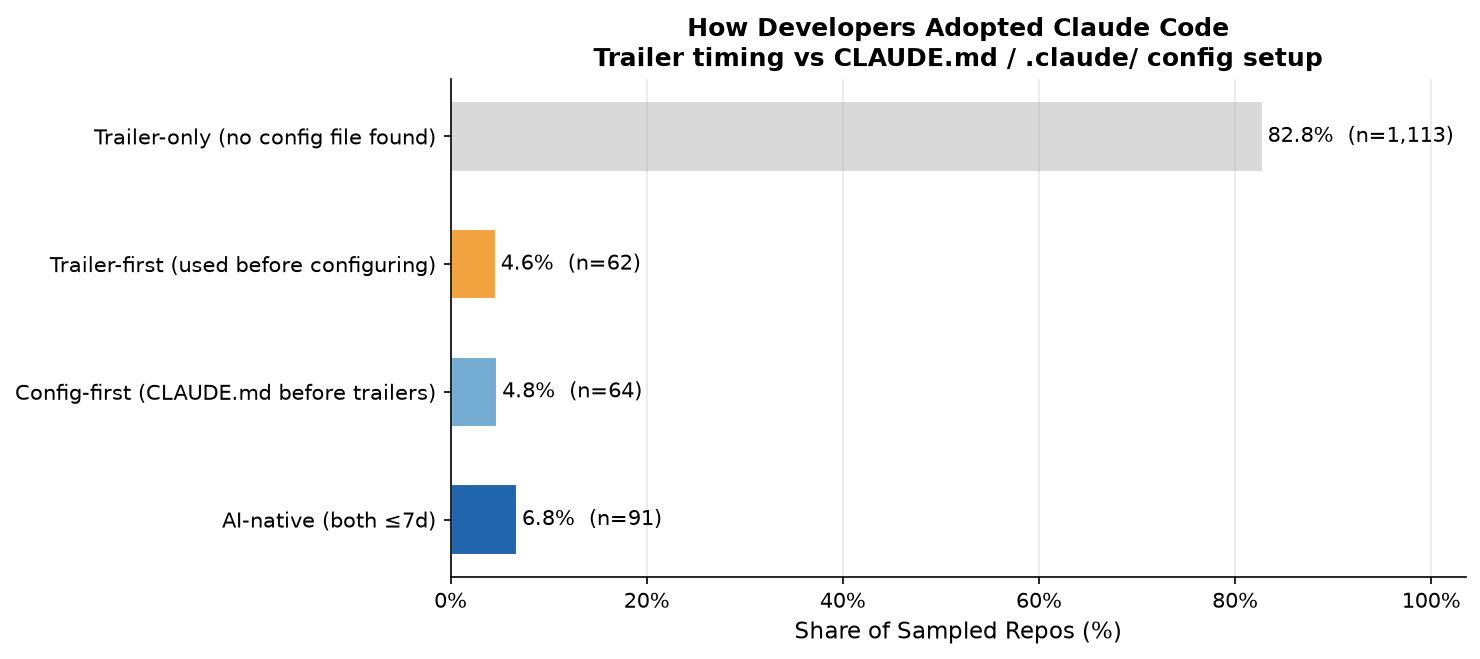
\includegraphics[width=\linewidth]{stage5/fig_adoption_pattern.png}\\
    \small\textit{E4 --- Adoption pattern distribution}
  \end{minipage}
\end{center}

\end{document}
